% =====================================================================
% 3. Area 1: core architectures (PRDL, Maria Martinez)
% Own blocks in depth: RNN (LSTM/GRU), RNN + attention, self-attention,
% Transformer (T11, T12; DECISIONS D17, D18; block notes 06 and 07).
% Dense and CNN (Oriana's blocks, T9, T10) summarised and attributed.
% Every number is a macro of numbers.tex.
% =====================================================================
\section{Area 1: core architectures}\label{sec:architectures}

The first area of the guidelines asks for the fundamental modules applied to a simple example
\cite{course_message_2011}. All families below read the same normalised 12-lead records, are trained
with the same loop and evaluated with the same protocol (Section~\ref{sec:evaluation}), so a difference
between them comes from the architecture. Each family was studied with an ablation grid on the
validation fold (three seeds per configuration, one factor changed at a time against a stated
reference) and one final model per family, chosen by a rule fixed before the runs and evaluated once on
the test fold. In the ablation tables, $\Delta$ is the mean paired difference with the reference trained
with the same seed, and ``better / worse'' counts the seeds whose paired 95\,\% interval lies wholly
above or below 0.

\subsection{Dense network and 1D CNN (Oriana's blocks, summarised)}\label{sec:dense-cnn}

The dense network and the CNN were designed, run and analysed by Oriana; I reviewed both blocks. The
dense network flattens the record into one vector, so each weight belongs to one lead and one instant:
nothing it learns at one moment of the record can be reused at another. It is the floor of the
comparison among real architectures, with a test macro AUROC of
\denseFinalTestMacroAurocMean{}~$\pm$~\denseFinalTestMacroAurocSd{} and
\denseFinalNParams{} parameters. The residual 1D CNN applies the same small filters along the whole
record (kernel 7 = 70\,ms at 100\,Hz) and pools globally at the end; it is the strongest family of the
project, with \cnnFinalTestMacroAurocMean{}~$\pm$~\cnnFinalTestMacroAurocSd{} on test and
\cnnFinalNParams{} parameters (\cnnDiffDenseMean{} above the dense network on average). This contrast is
the reference for my blocks: the question for recurrence and attention is how much they add, or lose,
with respect to local filters shared over time.
Table~\ref{tab:dense_ablations} shows Oriana's dense ablations, which also define the conventions of all
ablation tables of this report.

% Shared float (common/make_floats.py). Table: tables/dense_ablations.tex
\begin{table}[htbp]
\centering
\caption[Dense network: ablations (validation)]{Dense ablations on the validation fold: mean $\pm$ SD over seeds 42--44; $\Delta$ = mean paired difference with the baseline of the same seed; seeds better / worse = seeds whose paired 95\,\% patient-bootstrap interval lies wholly above / below 0.}
\label{tab:dense_ablations}
\small
\begin{adjustbox}{max width=\textwidth}
% Generated by src/dense_experiments.py from results/logs/dense_summary.json.
% Needs report/numbers.tex (alias "dense" in report/runs.json) and \usepackage{booktabs}.
\begin{tabular}{llrcrc}
\toprule
Factor & Configuration & Parameters & Val.\ macro AUROC & $\Delta$ vs.\ baseline & Seeds better / worse \\
\midrule
baseline & Baseline: z-score, BN, dropout 0.5, 2 $\times$ 256 & \denseParamsBase{} & \denseValAurocMeanBase{} $\pm$ \denseValAurocSdBase{} & --- & --- \\
\addlinespace
input scaling & No input z-score (raw mV) & \denseParamsNoNorm{} & \denseValAurocMeanNoNorm{} $\pm$ \denseValAurocSdNoNorm{} & \denseDiffMeanNoNorm{} & \denseNSeedsBetterNoNorm{} / \denseNSeedsWorseNoNorm{} of \denseNSeedsComparedNoNorm{} \\
\addlinespace
batch norm & No batch norm & \denseParamsNoBn{} & \denseValAurocMeanNoBn{} $\pm$ \denseValAurocSdNoBn{} & \denseDiffMeanNoBn{} & \denseNSeedsBetterNoBn{} / \denseNSeedsWorseNoBn{} of \denseNSeedsComparedNoBn{} \\
\addlinespace
input scaling $\times$ batch norm & No input z-score and no batch norm & \denseParamsNoNormNoBn{} & \denseValAurocMeanNoNormNoBn{} $\pm$ \denseValAurocSdNoNormNoBn{} & \denseDiffMeanNoNormNoBn{} & \denseNSeedsBetterNoNormNoBn{} / \denseNSeedsWorseNoNormNoBn{} of \denseNSeedsComparedNoNormNoBn{} \\
\addlinespace
dropout & No dropout & \denseParamsNoDropout{} & \denseValAurocMeanNoDropout{} $\pm$ \denseValAurocSdNoDropout{} & \denseDiffMeanNoDropout{} & \denseNSeedsBetterNoDropout{} / \denseNSeedsWorseNoDropout{} of \denseNSeedsComparedNoDropout{} \\
dropout & Dropout 0.2 & \denseParamsDropoutZeroTwo{} & \denseValAurocMeanDropoutZeroTwo{} $\pm$ \denseValAurocSdDropoutZeroTwo{} & \denseDiffMeanDropoutZeroTwo{} & \denseNSeedsBetterDropoutZeroTwo{} / \denseNSeedsWorseDropoutZeroTwo{} of \denseNSeedsComparedDropoutZeroTwo{} \\
\addlinespace
depth & 1 hidden layer (256) & \denseParamsDepthOne{} & \denseValAurocMeanDepthOne{} $\pm$ \denseValAurocSdDepthOne{} & \denseDiffMeanDepthOne{} & \denseNSeedsBetterDepthOne{} / \denseNSeedsWorseDepthOne{} of \denseNSeedsComparedDepthOne{} \\
depth & 3 hidden layers (256) & \denseParamsDepthThree{} & \denseValAurocMeanDepthThree{} $\pm$ \denseValAurocSdDepthThree{} & \denseDiffMeanDepthThree{} & \denseNSeedsBetterDepthThree{} / \denseNSeedsWorseDepthThree{} of \denseNSeedsComparedDepthThree{} \\
depth & 4 hidden layers (256) & \denseParamsDepthFour{} & \denseValAurocMeanDepthFour{} $\pm$ \denseValAurocSdDepthFour{} & \denseDiffMeanDepthFour{} & \denseNSeedsBetterDepthFour{} / \denseNSeedsWorseDepthFour{} of \denseNSeedsComparedDepthFour{} \\
\addlinespace
width & Width 64 (2 layers) & \denseParamsWidthSixFour{} & \denseValAurocMeanWidthSixFour{} $\pm$ \denseValAurocSdWidthSixFour{} & \denseDiffMeanWidthSixFour{} & \denseNSeedsBetterWidthSixFour{} / \denseNSeedsWorseWidthSixFour{} of \denseNSeedsComparedWidthSixFour{} \\
width & Width 1024 (2 layers) & \denseParamsWidthOneZeroTwoFour{} & \denseValAurocMeanWidthOneZeroTwoFour{} $\pm$ \denseValAurocSdWidthOneZeroTwoFour{} & \denseDiffMeanWidthOneZeroTwoFour{} & \denseNSeedsBetterWidthOneZeroTwoFour{} / \denseNSeedsWorseWidthOneZeroTwoFour{} of \denseNSeedsComparedWidthOneZeroTwoFour{} \\
\bottomrule
\end{tabular}

\end{adjustbox}
\end{table}


% ---------------------------------------------------------------------
\subsection{Recurrent networks: LSTM and GRU}\label{sec:rnn}

\paragraph{Theory.} A recurrent network reads a sequence one step at a time. Its hidden state at step
$t$ is a function of the current input and of the previous state, $h_t = f(x_t, h_{t-1})$, and the same
weights are applied at every step, so whatever the network learns about a pattern can be applied
wherever the pattern occurs. Training unfolds the network over the $T$ steps into a very deep
feed-forward network with shared weights, and the gradient of the loss with respect to an early input is
a product of many Jacobians (backpropagation through time). Such products tend to shrink or to grow
exponentially with the distance, so a plain recurrent network remembers recent inputs much better than
distant ones and its training can become unstable. Gated cells reduce the first problem: the LSTM keeps
a separate cell state updated additively through forget, input and output gates, and the GRU merges the
gates into an update and a reset gate, a design that is ``motivated by the LSTM unit but is much
simpler to compute and implement'' \cite{cho2014learning}. A large comparison of LSTM variants found
that none of them improves on the standard LSTM significantly \cite{greff2017lstm}, which the course
slides summarise as the variants being ``all about the same'' \cite{course_rnn_slides}. Against
exploding gradients we clip the total gradient norm, a remedy that has been shown to work well in
practice \cite{pascanu2013difficulty}.

\paragraph{Design (DECISIONS D17).} A recurrent network needs one vector per time step. In the baseline
the record is cut into 100 non-overlapping frames of 10 samples (100\,ms), and each step receives the
12 leads $\times$ 10 samples of one frame as a vector of 120 numbers. Framing shortens the sequence
(100 steps instead of 1000, so backpropagation through time is ten times shorter) without discarding any
sample, unlike downsampling. The baseline is a unidirectional LSTM with two layers of 128 units; its
final hidden state feeds dropout and a linear layer with five logits, the same head as the CNN
(\rnnParamsBase{} parameters). The ablations change one factor at a time (Table~\ref{tab:rnn_ablations}):
the cell (GRU), the depth, the direction (bidirectional), the readout (the mean of all hidden states, or
attention, Section~\ref{sec:rnn-attn}), and the input sequence: one raw sample per step
(\rnnStepsRaw{} steps) or a convolutional front end made of the first three blocks of the CNN, which
turns the record into \rnnStepsConv{} steps of 128 features (a CNN feature extractor followed by an
LSTM). Gradients are clipped at a total norm of \rnnGradClip{} in every configuration.

% Shared float (common/make_floats.py). Table: tables/rnn_ablations.tex
\begin{table}[htbp]
\centering
\caption[Recurrent networks: ablations (validation)]{RNN ablations on the validation fold (conventions of Table~\ref{tab:dense_ablations}; each row is compared with its own reference). Last 2\,s: share of the input sensitivity in the last 2\,s of the record (uniform: 0.2).}
\label{tab:rnn_ablations}
\small
\begin{adjustbox}{max width=\textwidth}
% Generated by src/rnn_experiments.py from results/logs/rnn_summary.json.
% Needs report/numbers.tex (alias "rnn" in report/runs.json) and \usepackage{booktabs}.
% Delta: paired difference with the reference trained with the same seed (the baseline unless the label says otherwise).
% Last 2 s: share of the input sensitivity in the last 2 s of the record (seed 42; 0.2 if uniform).
\begin{tabular}{llrrcrcc}
\toprule
Factor & Configuration & Parameters & Steps & Val.\ macro AUROC & $\Delta$ vs.\ reference & Seeds better / worse & Last 2\,s \\
\midrule
baseline & Baseline: LSTM 2 $\times$ 128, 100 frames, last state & \rnnParamsBase{} & \rnnStepsBase{} & \rnnValAurocMeanBase{} $\pm$ \rnnValAurocSdBase{} & --- & --- & \rnnSensLastBase{} \\
\addlinespace
cell & GRU instead of LSTM & \rnnParamsGru{} & \rnnStepsGru{} & \rnnValAurocMeanGru{} $\pm$ \rnnValAurocSdGru{} & \rnnDiffMeanGru{} & \rnnNSeedsBetterGru{} / \rnnNSeedsWorseGru{} of \rnnNSeedsComparedGru{} & \rnnSensLastGru{} \\
\addlinespace
depth & 1 recurrent layer & \rnnParamsLayersOne{} & \rnnStepsLayersOne{} & \rnnValAurocMeanLayersOne{} $\pm$ \rnnValAurocSdLayersOne{} & \rnnDiffMeanLayersOne{} & \rnnNSeedsBetterLayersOne{} / \rnnNSeedsWorseLayersOne{} of \rnnNSeedsComparedLayersOne{} & \rnnSensLastLayersOne{} \\
\addlinespace
direction & Bidirectional & \rnnParamsBi{} & \rnnStepsBi{} & \rnnValAurocMeanBi{} $\pm$ \rnnValAurocSdBi{} & \rnnDiffMeanBi{} & \rnnNSeedsBetterBi{} / \rnnNSeedsWorseBi{} of \rnnNSeedsComparedBi{} & \rnnSensLastBi{} \\
\addlinespace
readout & Mean of the states over time & \rnnParamsMean{} & \rnnStepsMean{} & \rnnValAurocMeanMean{} $\pm$ \rnnValAurocSdMean{} & \rnnDiffMeanMean{} & \rnnNSeedsBetterMean{} / \rnnNSeedsWorseMean{} of \rnnNSeedsComparedMean{} & \rnnSensLastMean{} \\
readout & Additive attention & \rnnParamsAttn{} & \rnnStepsAttn{} & \rnnValAurocMeanAttn{} $\pm$ \rnnValAurocSdAttn{} & \rnnDiffMeanAttn{} & \rnnNSeedsBetterAttn{} / \rnnNSeedsWorseAttn{} of \rnnNSeedsComparedAttn{} & \rnnSensLastAttn{} \\
\addlinespace
attention score & Notebook score $\tanh(w^\top h+b)$ (vs. additive) & \rnnParamsAttnTanh{} & \rnnStepsAttnTanh{} & \rnnValAurocMeanAttnTanh{} $\pm$ \rnnValAurocSdAttnTanh{} & \rnnDiffMeanAttnTanh{} & \rnnNSeedsBetterAttnTanh{} / \rnnNSeedsWorseAttnTanh{} of \rnnNSeedsComparedAttnTanh{} & \rnnSensLastAttnTanh{} \\
\addlinespace
attention $\times$ cell & GRU + attention (vs. GRU) & \rnnParamsGruAttn{} & \rnnStepsGruAttn{} & \rnnValAurocMeanGruAttn{} $\pm$ \rnnValAurocSdGruAttn{} & \rnnDiffMeanGruAttn{} & \rnnNSeedsBetterGruAttn{} / \rnnNSeedsWorseGruAttn{} of \rnnNSeedsComparedGruAttn{} & \rnnSensLastGruAttn{} \\
\addlinespace
attention $\times$ direction & Bidirectional + attention (vs. bidirectional) & \rnnParamsBiAttn{} & \rnnStepsBiAttn{} & \rnnValAurocMeanBiAttn{} $\pm$ \rnnValAurocSdBiAttn{} & \rnnDiffMeanBiAttn{} & \rnnNSeedsBetterBiAttn{} / \rnnNSeedsWorseBiAttn{} of \rnnNSeedsComparedBiAttn{} & \rnnSensLastBiAttn{} \\
\addlinespace
input & Convolutional front end (125 steps) & \rnnParamsConv{} & \rnnStepsConv{} & \rnnValAurocMeanConv{} $\pm$ \rnnValAurocSdConv{} & \rnnDiffMeanConv{} & \rnnNSeedsBetterConv{} / \rnnNSeedsWorseConv{} of \rnnNSeedsComparedConv{} & \rnnSensLastConv{} \\
\addlinespace
sequence length & Raw samples (1000 steps) & \rnnParamsRaw{} & \rnnStepsRaw{} & \rnnValAurocMeanRaw{} $\pm$ \rnnValAurocSdRaw{} & \rnnDiffMeanRaw{} & \rnnNSeedsBetterRaw{} / \rnnNSeedsWorseRaw{} of \rnnNSeedsComparedRaw{} & \rnnSensLastRaw{} \\
\addlinespace
attention $\times$ sequence length & 1000 steps + attention (vs. 1000 steps) & \rnnParamsRawAttn{} & \rnnStepsRawAttn{} & \rnnValAurocMeanRawAttn{} $\pm$ \rnnValAurocSdRawAttn{} & \rnnDiffMeanRawAttn{} & \rnnNSeedsBetterRawAttn{} / \rnnNSeedsWorseRawAttn{} of \rnnNSeedsComparedRawAttn{} & \rnnSensLastRawAttn{} \\
\bottomrule
\end{tabular}

\end{adjustbox}
\end{table}

% Shared float (common/make_floats.py). Figure: figures/rnn_ablations.pdf
\begin{figure}[htbp]
\centering
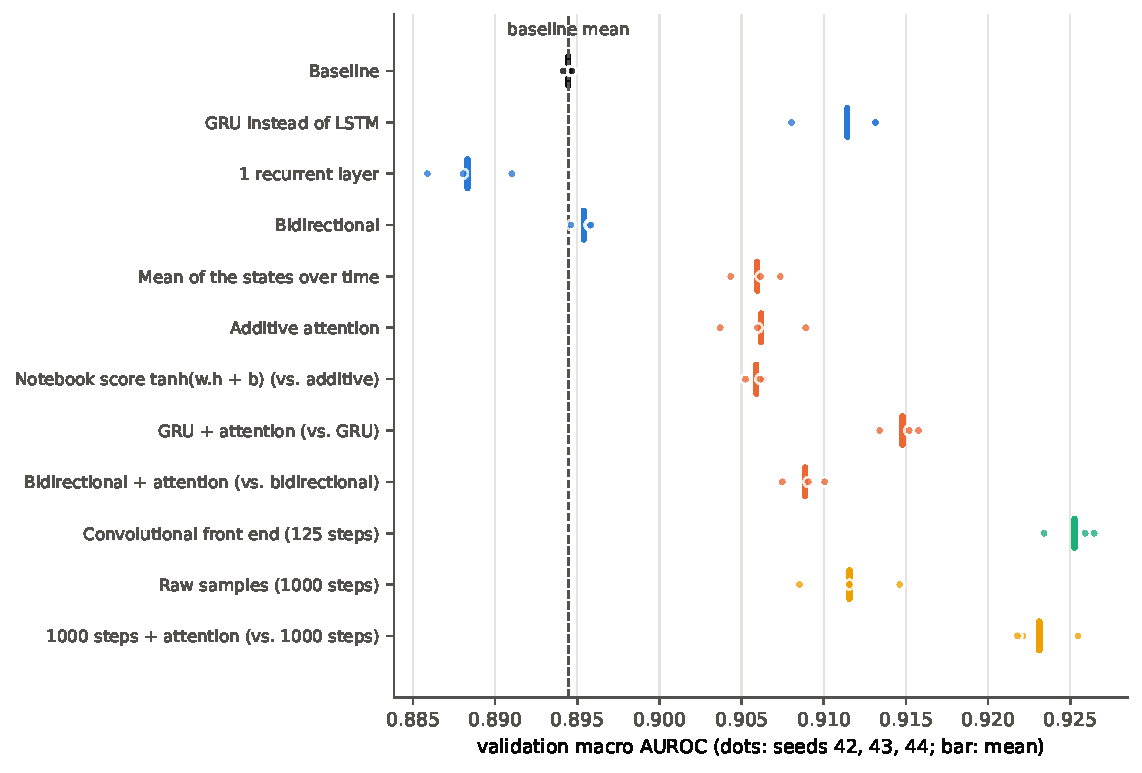
\includegraphics[width=\textwidth,height=0.42\textheight,keepaspectratio]{figures/rnn_ablations.pdf}
\caption[Recurrent networks: ablations]{RNN ablations: validation macro AUROC (dots: seeds 42, 43, 44; bar: mean; dashed line: baseline mean). Rows marked ``vs.'' are compared with their own reference.}
\label{fig:rnn_ablations}
\end{figure}


\paragraph{Results.} Table~\ref{tab:rnn_ablations} and Figure~\ref{fig:rnn_ablations} give the
validation results; my reading of them is the following.
\begin{enumerate}[leftmargin=1.4em,itemsep=2pt]
  \item \textbf{Using every hidden state matters more than the cell or the direction.} Replacing the last
        state by the mean of all states changes the validation AUROC by \rnnDiffMeanMean{} (better in
        \rnnNSeedsBetterMean{} of \rnnNSeedsComparedMean{} seeds); a bidirectional network that still
        reads only its final states changes it by \rnnDiffMeanBi{} (\rnnNSeedsBetterBi{} better,
        \rnnNSeedsWorseBi{} worse). The final state is a bottleneck: whatever the network saw early in the
        record must survive many updates to reach it.
  \item \textbf{The GRU beats the LSTM} by \rnnDiffMeanGru{} (\rnnNSeedsBetterGru{} of
        \rnnNSeedsComparedGru{} seeds), with fewer parameters (\rnnParamsGru{} against \rnnParamsBase{}),
        in fewer epochs (best epoch \onedec{\rnnBestEpochMeanGru} against \onedec{\rnnBestEpochMeanBase})
        and with a lower training loss at epoch 5 (\rnnTrainLossEpFiveDiffMeanGru{}). This does not
        contradict the literature above, which concerns variants of the LSTM, not the GRU. My explanation,
        not tested, is that a cell with fewer gates is easier to fit with the
        \edaNLabelledTrain{} training records we have.
  \item \textbf{1000 raw steps are better than 100 frames} (\rnnDiffMeanRaw{}, \rnnNSeedsBetterRaw{} of
        \rnnNSeedsComparedRaw{} seeds), against what we expected. They are much harder to optimise, as
        backpropagation through time predicts: the training loss at epoch 5 is higher by
        \rnnTrainLossEpFiveDiffMeanRaw{}, the best epoch moves from \onedec{\rnnBestEpochMeanBase} to
        \onedec{\rnnBestEpochMeanRaw} and a run takes \onedec{\rnnTrainTimeMinMeanRaw}\,min instead of
        \onedec{\rnnTrainTimeMinMeanBase}\,min (Figure~\ref{fig:rnn_curves}c). My explanation, a
        hypothesis: a frame is flattened into one vector, so a QRS complex is seen by different weights
        depending on where it falls inside the frame, whereas with one sample per step the same recurrent
        weights process every sample, which is the weight sharing over time of the CNN.
  \item \textbf{The convolutional front end is the best configuration} (\rnnDiffMeanConv{},
        \rnnNSeedsBetterConv{} of \rnnNSeedsComparedConv{} seeds). Local filters shared over time extract
        beat-level features and the LSTM only has to combine \rnnStepsConv{} of them. Points 3 and 4 point
        in the same direction: what helps is sharing weights over time, more than recurrence itself.
\end{enumerate}

% Shared float (common/make_floats.py). Figure: figures/rnn_curves.pdf
\begin{figure}[htbp]
\centering
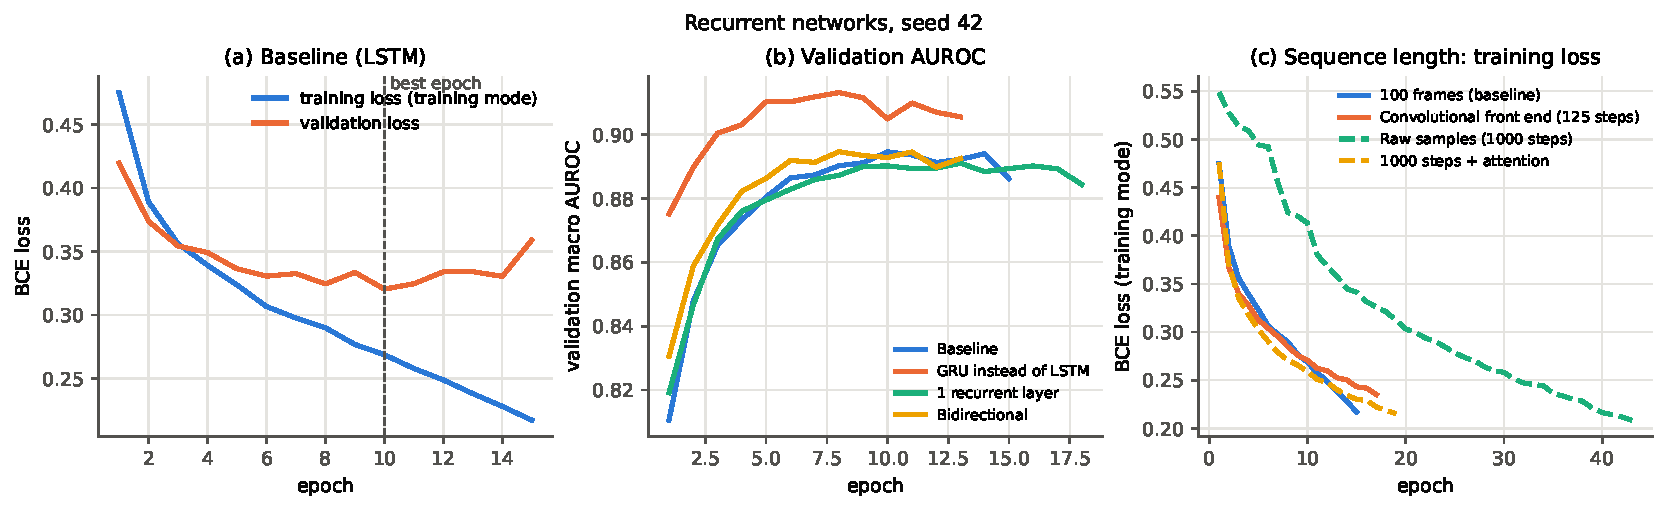
\includegraphics[width=\textwidth,height=0.42\textheight,keepaspectratio]{figures/rnn_curves.pdf}
\caption[Recurrent networks: learning curves]{Recurrent networks, seed 42. (a) LSTM baseline losses. (b) Validation macro AUROC of the baseline, GRU, one recurrent layer and bidirectional LSTM. (c) Training loss with 100 frames, the convolutional front end, 1000 raw steps and 1000 steps with attention.}
\label{fig:rnn_curves}
\end{figure}


\paragraph{Which part of the record the output depends on.} To see the short memory directly, I
measured the gradient of the output with respect to the input at every instant, $|\partial\,
\mathrm{logit}/\partial x(\text{lead}, t)|$, summed over leads and averaged over classes and
\rnnSensNRecords{} validation records, and normalised it over the 10\,s
(Figure~\ref{fig:rnn_time_gradient}). With the last state of the unidirectional LSTM,
\rnnSensLastBase{} of the sensitivity falls in the last 2\,s of the record, against 0.2 if it were
uniform, half of it in the last \rnnSensHalfWindowSBase\,s, and only \rnnSensFirstBase{} in the first
2\,s: the network mostly looks at the end of the record, as vanishing gradients predict. With 1000 raw
steps the pattern is the same (\rnnSensLastRaw{} in the last 2\,s). A bidirectional network weighs both
ends (\rnnSensFirstBi{} in the first 2\,s, \rnnSensLastBi{} in the last), and the mean and attention
readouts are almost uniform except for a drop in the last second (\rnnSensLastMean{} and
\rnnSensLastAttn{} in the last 2\,s). That drop follows from the structure of a unidirectional network:
the input at time $t$ can only change the states from $t$ onwards, so the last samples affect few of the
states being averaged. The spread of the sensitivity is not what improves the result by itself: the
bidirectional network spreads it but gains nothing.

% Shared float (common/make_floats.py). Figure: figures/rnn_time_gradient.pdf
\begin{figure}[htbp]
\centering
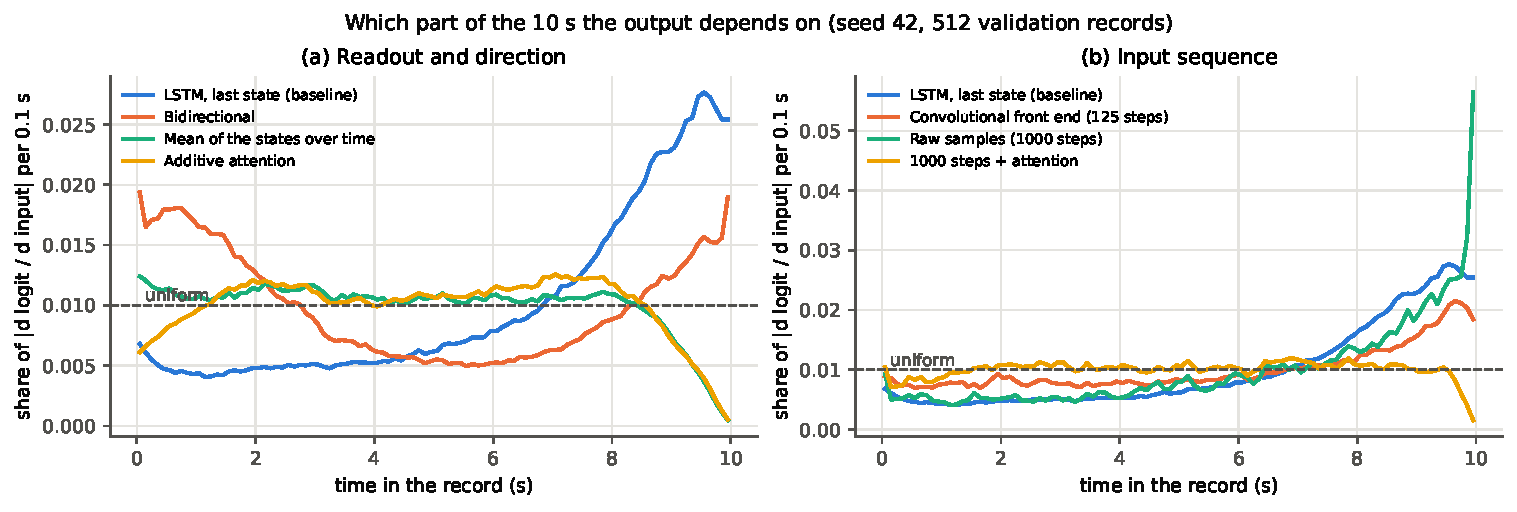
\includegraphics[width=\textwidth,height=0.42\textheight,keepaspectratio]{figures/rnn_time_gradient.pdf}
\caption[Recurrent networks: input sensitivity over time]{Which part of the 10\,s the output depends on (share of the input gradient per 0.1\,s, seed 42, 512 validation records; dashed: uniform). (a) Readout and direction. (b) Input sequence.}
\label{fig:rnn_time_gradient}
\end{figure}


% ---------------------------------------------------------------------
\subsection{RNN + attention}\label{sec:rnn-attn}

\paragraph{Theory.} Attention was introduced in neural translation to remove the bottleneck of a single
summary vector: instead of the encoder's last state, the decoder receives a weighted mean of all encoder
states, with weights given by an alignment model that ``scores how well the inputs around position $j$
and the output at position $i$ match'' \cite{bahdanau2015neural}. A classifier has no decoder, so the
query becomes a learned vector, the same for every record, as in the class notebook. For each step a
score $e_t$ is computed from the hidden state $h_t$; a softmax over time turns the scores into weights
$\alpha_t \ge 0$ that sum to 1; and the context vector $\sum_t \alpha_t h_t$ replaces the last state as
the input of the classifier. Our score is additive, $e_t = v^\top \tanh(W h_t + b)$, a feed-forward
network with one hidden layer of 64 units. The ablation \texttt{attn\_tanh} uses the notebook's score,
$e_t = \tanh(w^\top h_t + b)$. Its scores lie in $[-1, 1]$, so no weight can exceed
$1/(1 + (T-1)e^{-2})$, which is \rnnAttnMaxBoundAttnTanh{} for $T = 100$ against a uniform weight of
\rnnAttnUniformAttnTanh{}: this score can never concentrate on a few steps.

\paragraph{Design.} RNN + attention is a model of its own (decision D6 after the guidelines of 20/11),
with its own selection rule: the final RNN + attention is the best of the five attention configurations
(\texttt{attn}, \texttt{attn\_tanh}, \texttt{gru\_attn}, \texttt{bi\_attn}, \texttt{raw\_attn}). Three of
them cross attention with another factor, to test a prediction of the theory: if attention removes the
bottleneck of the last state, it should help most where that state struggles, with 1000 steps and with a
unidirectional network.

\paragraph{Results.}
\begin{enumerate}[leftmargin=1.4em,itemsep=2pt]
  \item \textbf{Attention helps as much as the mean, not more.} Additive attention changes the validation
        AUROC by \rnnDiffMeanAttn{} with respect to the last state (\rnnNSeedsBetterAttn{} of
        \rnnNSeedsComparedAttn{} seeds), the same gain as mean pooling (\rnnDiffMeanMean{}); the two
        were not compared directly, but their means are \rnnValAurocMeanAttn{} and
        \rnnValAurocMeanMean{}.
  \item \textbf{The weights are spread out} (Table~\ref{tab:rnn_attention}): normalised entropy
        \rnnAttnEntropyNormAttn{} (1 = uniform), about \intval{\rnnAttnEffectiveStepsAttn} of the 100
        steps effectively attended, and a largest weight of \rnnAttnMaxWeightAttn{} against a uniform
        \rnnAttnUniformAttn{}. Here attention behaves like a learned mean.
  \item \textbf{The notebook score changes nothing in the result} (\rnnDiffMeanAttnTanh{},
        \rnnNSeedsBetterAttnTanh{} better, \rnnNSeedsWorseAttnTanh{} worse); its weights are even flatter
        (entropy \rnnAttnEntropyNormAttnTanh{}, largest weight \rnnAttnMaxWeightAttnTanh{}, far below its
        bound), so it is almost exactly mean pooling.
  \item \textbf{The prediction of the theory is not supported.} Attention adds \rnnDiffMeanRawAttn{} at
        1000 steps, \rnnDiffMeanAttn{} at 100, \rnnDiffMeanBiAttn{} to the bidirectional network and
        \rnnDiffMeanGruAttn{} to the GRU (\rnnNSeedsBetterGruAttn{} of \rnnNSeedsComparedGruAttn{} seeds).
        The bottleneck is real, but in this task averaging removes it just as well, and the GRU, whose last
        state already reaches \rnnValAurocMeanGru{}, leaves least to gain.
\end{enumerate}

% Shared float (common/make_floats.py). Table: tables/rnn_attention.tex
\begin{table}[htbp]
\centering
\caption[RNN + attention: attention statistics]{Attention statistics of the RNN + attention models (seed 42, validation).}
\label{tab:rnn_attention}
\small
\begin{adjustbox}{max width=\textwidth}
% Generated by src/rnn_experiments.py from results/logs/rnn_summary.json.
% Attention weights of the seed-42 model of each configuration over the whole validation fold.
% Entropy: H(alpha) / log T (1 = uniform weights). Spearman: correlation of the weights with the step's signal activity.
\begin{tabular}{lrcccc}
\toprule
Configuration & Steps $T$ & Uniform $1/T$ & Mean largest weight & Norm.\ entropy (eff.\ steps) & Spearman with activity \\
\midrule
Additive attention & \rnnAttnStepsAttn{} & \rnnAttnUniformAttn{} & \rnnAttnMaxWeightAttn{} & \rnnAttnEntropyNormAttn{} (\rnnAttnEffectiveStepsAttn{}) & \rnnAttnSpearmanActivityAttn{} \\
Notebook score $\tanh(w^\top h+b)$ (vs. additive) & \rnnAttnStepsAttnTanh{} & \rnnAttnUniformAttnTanh{} & \rnnAttnMaxWeightAttnTanh{} (bound \rnnAttnMaxBoundAttnTanh{}) & \rnnAttnEntropyNormAttnTanh{} (\rnnAttnEffectiveStepsAttnTanh{}) & \rnnAttnSpearmanActivityAttnTanh{} \\
GRU + attention (vs. GRU) & \rnnAttnStepsGruAttn{} & \rnnAttnUniformGruAttn{} & \rnnAttnMaxWeightGruAttn{} & \rnnAttnEntropyNormGruAttn{} (\rnnAttnEffectiveStepsGruAttn{}) & \rnnAttnSpearmanActivityGruAttn{} \\
Bidirectional + attention (vs. bidirectional) & \rnnAttnStepsBiAttn{} & \rnnAttnUniformBiAttn{} & \rnnAttnMaxWeightBiAttn{} & \rnnAttnEntropyNormBiAttn{} (\rnnAttnEffectiveStepsBiAttn{}) & \rnnAttnSpearmanActivityBiAttn{} \\
1000 steps + attention (vs. 1000 steps) & \rnnAttnStepsRawAttn{} & \rnnAttnUniformRawAttn{} & \rnnAttnMaxWeightRawAttn{} & \rnnAttnEntropyNormRawAttn{} (\rnnAttnEffectiveStepsRawAttn{}) & \rnnAttnSpearmanActivityRawAttn{} \\
\bottomrule
\end{tabular}

\end{adjustbox}
\end{table}

% Shared float (common/make_floats.py). Figure: figures/rnn_attention.pdf
\begin{figure}[htbp]
\centering
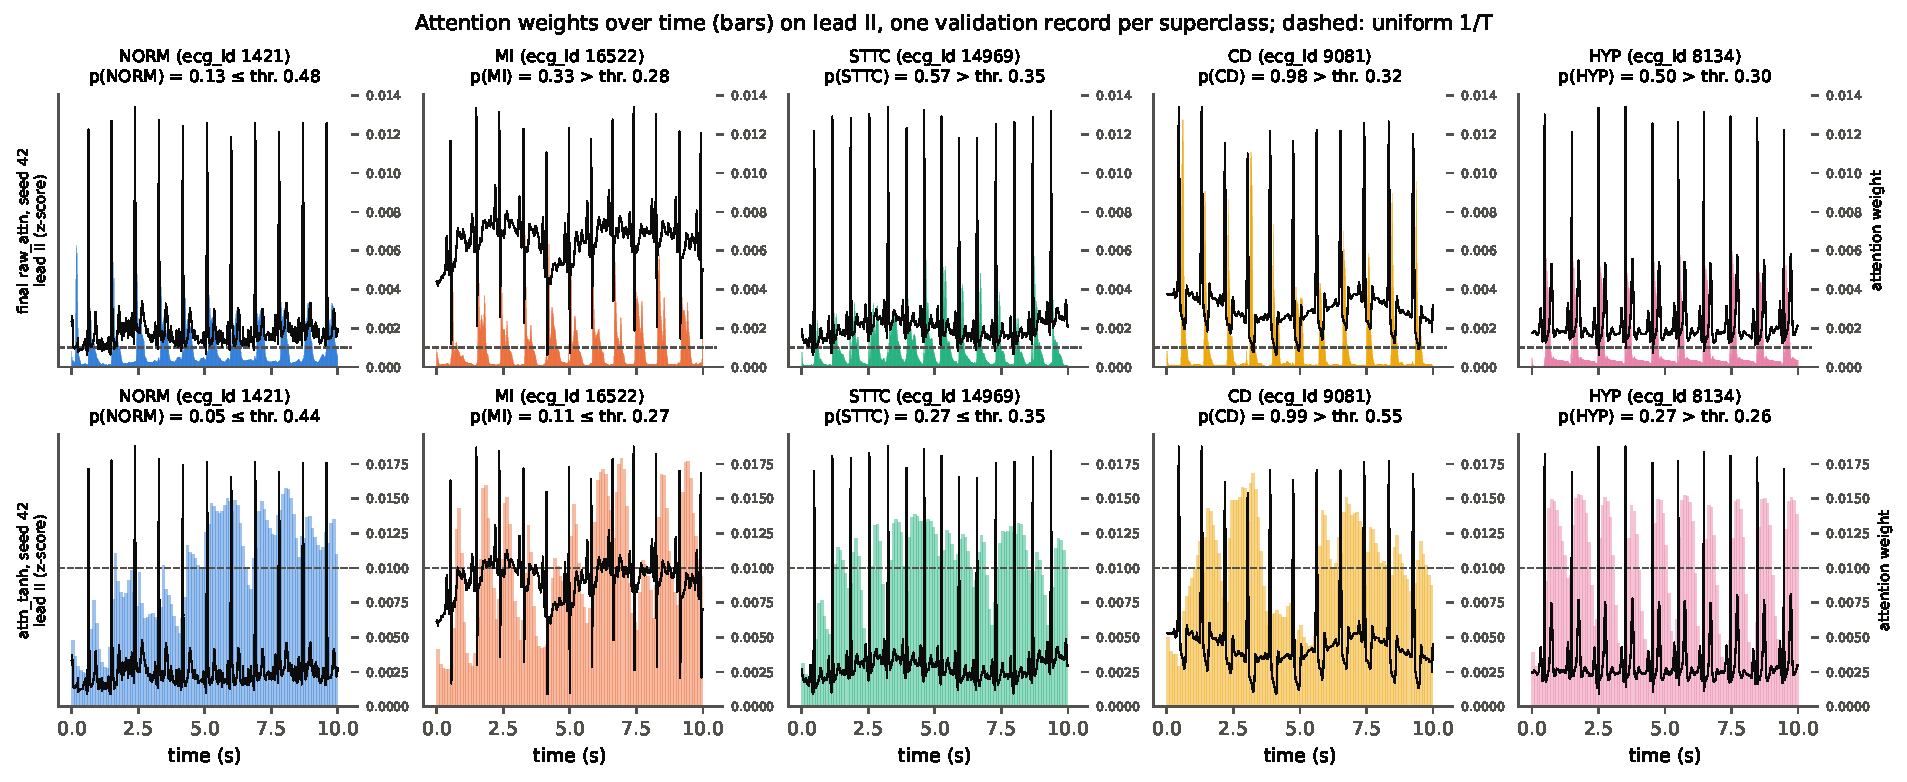
\includegraphics[width=\textwidth,height=0.42\textheight,keepaspectratio]{figures/rnn_attention.pdf}
\caption[RNN + attention: attention weights over time]{Attention weights over time (bars) on lead II for one validation record per superclass: final RNN + attention (\texttt{raw\_attn}, top) and the notebook tanh score over 100 frames (bottom); dashed: uniform weight $1/T$. Titles: predicted probability and threshold.}
\label{fig:rnn_attention}
\end{figure}


\paragraph{Attention over the ECG.} Figure~\ref{fig:rnn_attention} draws the weights of the final RNN +
attention (\texttt{raw\_attn}, 1000 steps) over lead II of one validation record per superclass. In all
five records the weights rise and fall with the heartbeat, one bump per beat around the QRS complexes.
This is a visual observation: the correlation between the weights and our activity proxy (mean absolute
sample-to-sample change), fixed before the runs, is only \rnnAttnSpearmanActivityRawAttn{} for this model
and does not capture the alignment. Possible reasons, not tested: the bump may sit just after the QRS (a
state can only reflect a QRS after reading it), or the ranks of the many near-zero weights between beats
may be noise. I therefore do not use the correlation as evidence that attention follows the QRS. The
second row (notebook score, 100 steps) is periodic too but much flatter, on a different scale (uniform
weight \rnnAttnUniformAttnTanh{} instead of \rnnAttnUniformRawAttn{}). The predicted probabilities are in
the column titles; one of the five records (NORM) is missed by the final model, and the weights must be
read with that in mind.

\paragraph{Final recurrent models.} By the rules of D17, the final RNN is \texttt{conv}, the best of all
twelve configurations, and the final RNN + attention is \texttt{raw\_attn}, the best attention
configuration (Table~\ref{tab:rnn_final}). On test, \texttt{conv} reaches
\rnnFinalTestMacroAurocMean{}~$\pm$~\rnnFinalTestMacroAurocSd{} and \texttt{raw\_attn}
\rnnAttnfinalTestMacroAurocMean{}~$\pm$~\rnnAttnfinalTestMacroAurocSd{}; their paired difference is
\rnnDiffAttnFinalMean{} and no seed separates them (\rnnNSeedsBetterAttnFinal{} better,
\rnnNSeedsWorseAttnFinal{} worse). Two caveats must be stated. First, the final RNN is a hybrid: its
comparison with the CNN is ``CNN'' against ``first half of the CNN + LSTM'', where the recurrent part
replaces the last convolutional block and the global pooling. It does slightly worse: \rnnDiffCnnMean{}
on average, worse in \rnnNSeedsWorseCnn{} of \rnnNSeedsComparedCnn{} seeds, with a similar size
(\rnnFinalNParams{} against \cnnFinalNParams{} parameters). Second, unlike the dense and CNN blocks, here
the rule selected a configuration that is clearly better than its baseline (point 4 of the results), but
the two final models cannot be told apart.

% Shared float (common/make_floats.py). Table: tables/rnn_final.tex
\begin{table}[htbp]
\centering
\caption[Recurrent networks: final models (test)]{Final RNN (\texttt{conv}) and RNN + attention (\texttt{raw\_attn}) on the test fold, with the final CNN, Dense and trivial models.}
\label{tab:rnn_final}
\small
\begin{adjustbox}{max width=\textwidth}
% Generated by src/rnn_experiments.py from results/logs/rnn_summary.json.
% Needs report/numbers.tex (aliases "rnn", "trivial", "cnn", "dense").
\begin{tabular}{lcccccc}
\toprule
 & \multicolumn{2}{c}{RNN (final)} & RNN + attention (final) & CNN (final) & Dense (final) & Trivial \\
\cmidrule(lr){2-3}
Test AUROC & First seed [95\% CI] & Mean $\pm$ SD (seeds) & Mean $\pm$ SD & Mean $\pm$ SD & Mean $\pm$ SD &  \\
\midrule
Macro & \rnnFinalFirstTestMacroAuroc{} [\rnnFinalFirstTestMacroAurocLo{}, \rnnFinalFirstTestMacroAurocHi{}] & \rnnFinalTestMacroAurocMean{} $\pm$ \rnnFinalTestMacroAurocSd{} & \rnnAttnfinalTestMacroAurocMean{} $\pm$ \rnnAttnfinalTestMacroAurocSd{} & \cnnFinalTestMacroAurocMean{} $\pm$ \cnnFinalTestMacroAurocSd{} & \denseFinalTestMacroAurocMean{} $\pm$ \denseFinalTestMacroAurocSd{} & \trivialTestMacroAuroc{} \\
\midrule
NORM & \rnnFinalFirstTestAurocNORM{} [\rnnFinalFirstTestAurocNORMLo{}, \rnnFinalFirstTestAurocNORMHi{}] & \rnnFinalTestAurocNORMMean{} $\pm$ \rnnFinalTestAurocNORMSd{} & \rnnAttnfinalTestAurocNORMMean{} $\pm$ \rnnAttnfinalTestAurocNORMSd{} & \cnnFinalTestAurocNORMMean{} $\pm$ \cnnFinalTestAurocNORMSd{} & \denseFinalTestAurocNORMMean{} $\pm$ \denseFinalTestAurocNORMSd{} & \trivialTestAurocNORM{} \\
MI & \rnnFinalFirstTestAurocMI{} [\rnnFinalFirstTestAurocMILo{}, \rnnFinalFirstTestAurocMIHi{}] & \rnnFinalTestAurocMIMean{} $\pm$ \rnnFinalTestAurocMISd{} & \rnnAttnfinalTestAurocMIMean{} $\pm$ \rnnAttnfinalTestAurocMISd{} & \cnnFinalTestAurocMIMean{} $\pm$ \cnnFinalTestAurocMISd{} & \denseFinalTestAurocMIMean{} $\pm$ \denseFinalTestAurocMISd{} & \trivialTestAurocMI{} \\
STTC & \rnnFinalFirstTestAurocSTTC{} [\rnnFinalFirstTestAurocSTTCLo{}, \rnnFinalFirstTestAurocSTTCHi{}] & \rnnFinalTestAurocSTTCMean{} $\pm$ \rnnFinalTestAurocSTTCSd{} & \rnnAttnfinalTestAurocSTTCMean{} $\pm$ \rnnAttnfinalTestAurocSTTCSd{} & \cnnFinalTestAurocSTTCMean{} $\pm$ \cnnFinalTestAurocSTTCSd{} & \denseFinalTestAurocSTTCMean{} $\pm$ \denseFinalTestAurocSTTCSd{} & \trivialTestAurocSTTC{} \\
CD & \rnnFinalFirstTestAurocCD{} [\rnnFinalFirstTestAurocCDLo{}, \rnnFinalFirstTestAurocCDHi{}] & \rnnFinalTestAurocCDMean{} $\pm$ \rnnFinalTestAurocCDSd{} & \rnnAttnfinalTestAurocCDMean{} $\pm$ \rnnAttnfinalTestAurocCDSd{} & \cnnFinalTestAurocCDMean{} $\pm$ \cnnFinalTestAurocCDSd{} & \denseFinalTestAurocCDMean{} $\pm$ \denseFinalTestAurocCDSd{} & \trivialTestAurocCD{} \\
HYP & \rnnFinalFirstTestAurocHYP{} [\rnnFinalFirstTestAurocHYPLo{}, \rnnFinalFirstTestAurocHYPHi{}] & \rnnFinalTestAurocHYPMean{} $\pm$ \rnnFinalTestAurocHYPSd{} & \rnnAttnfinalTestAurocHYPMean{} $\pm$ \rnnAttnfinalTestAurocHYPSd{} & \cnnFinalTestAurocHYPMean{} $\pm$ \cnnFinalTestAurocHYPSd{} & \denseFinalTestAurocHYPMean{} $\pm$ \denseFinalTestAurocHYPSd{} & \trivialTestAurocHYP{} \\
\midrule
$\Delta$ macro RNN vs.\ CNN, seed 42 & \rnnDiffCnnSFourTwo{} [\rnnDiffCnnLoSFourTwo{}, \rnnDiffCnnHiSFourTwo{}] & & & & & \\
$\Delta$ macro RNN vs.\ CNN, seed 43 & \rnnDiffCnnSFourThree{} [\rnnDiffCnnLoSFourThree{}, \rnnDiffCnnHiSFourThree{}] & & & & & \\
$\Delta$ macro RNN vs.\ CNN, seed 44 & \rnnDiffCnnSFourFour{} [\rnnDiffCnnLoSFourFour{}, \rnnDiffCnnHiSFourFour{}] & & & & & \\
$\Delta$ macro RNN vs.\ Dense, seed 42 & \rnnDiffDenseSFourTwo{} [\rnnDiffDenseLoSFourTwo{}, \rnnDiffDenseHiSFourTwo{}] & & & & & \\
$\Delta$ macro RNN vs.\ Dense, seed 43 & \rnnDiffDenseSFourThree{} [\rnnDiffDenseLoSFourThree{}, \rnnDiffDenseHiSFourThree{}] & & & & & \\
$\Delta$ macro RNN vs.\ Dense, seed 44 & \rnnDiffDenseSFourFour{} [\rnnDiffDenseLoSFourFour{}, \rnnDiffDenseHiSFourFour{}] & & & & & \\
$\Delta$ macro RNN vs.\ trivial, seed 42 & \rnnDiffTrivialSFourTwo{} [\rnnDiffTrivialLoSFourTwo{}, \rnnDiffTrivialHiSFourTwo{}] & & & & & \\
$\Delta$ macro RNN vs.\ trivial, seed 43 & \rnnDiffTrivialSFourThree{} [\rnnDiffTrivialLoSFourThree{}, \rnnDiffTrivialHiSFourThree{}] & & & & & \\
$\Delta$ macro RNN vs.\ trivial, seed 44 & \rnnDiffTrivialSFourFour{} [\rnnDiffTrivialLoSFourFour{}, \rnnDiffTrivialHiSFourFour{}] & & & & & \\
$\Delta$ macro RNN + att.\ vs.\ RNN, seed 42 & \rnnDiffAttnFinalSFourTwo{} [\rnnDiffAttnFinalLoSFourTwo{}, \rnnDiffAttnFinalHiSFourTwo{}] & & & & & \\
$\Delta$ macro RNN + att.\ vs.\ RNN, seed 43 & \rnnDiffAttnFinalSFourThree{} [\rnnDiffAttnFinalLoSFourThree{}, \rnnDiffAttnFinalHiSFourThree{}] & & & & & \\
$\Delta$ macro RNN + att.\ vs.\ RNN, seed 44 & \rnnDiffAttnFinalSFourFour{} [\rnnDiffAttnFinalLoSFourFour{}, \rnnDiffAttnFinalHiSFourFour{}] & & & & & \\
$\Delta$ macro RNN + att.\ vs.\ CNN, seed 42 & \rnnDiffAttnCnnSFourTwo{} [\rnnDiffAttnCnnLoSFourTwo{}, \rnnDiffAttnCnnHiSFourTwo{}] & & & & & \\
$\Delta$ macro RNN + att.\ vs.\ CNN, seed 43 & \rnnDiffAttnCnnSFourThree{} [\rnnDiffAttnCnnLoSFourThree{}, \rnnDiffAttnCnnHiSFourThree{}] & & & & & \\
$\Delta$ macro RNN + att.\ vs.\ CNN, seed 44 & \rnnDiffAttnCnnSFourFour{} [\rnnDiffAttnCnnLoSFourFour{}, \rnnDiffAttnCnnHiSFourFour{}] & & & & & \\
\bottomrule
\end{tabular}

\end{adjustbox}
\end{table}


% ---------------------------------------------------------------------
\subsection{Self-attention, step by step}\label{sec:selfattn}

\paragraph{Theory.} Self-attention lets every element of a sequence look at every other one. Each token
$x_i$ is projected into a query $q_i = x_i W_Q$, a key $k_i = x_i W_K$ and a value $v_i = x_i W_V$; the
weights of query $i$ are $\mathrm{softmax}_j(q_i \cdot k_j / \sqrt{d_k})$ and its output is the weighted
mean of the values. This is the ``Scaled Dot-Product Attention'' of the Transformer
\cite{vaswani2017attention}; the division by $\sqrt{d_k}$ keeps the dot products from growing with the
dimension and saturating the softmax. Multi-head attention runs several of these in parallel on smaller
projections and mixes their outputs with a matrix $W_O$, which ``allows the model to jointly attend to
information from different representation subspaces at different positions''
\cite{vaswani2017attention}. Compared with RNN + attention, the weights come from comparing tokens with
each other, not with one learned query, and nothing is sequential: all tokens are processed at once.

\paragraph{Design (DECISIONS D18).} The tokens are the same 100 patches of 10 samples as the RNN frames;
one linear layer (120 $\rightarrow$ 128) is the patch embedding, so ``attention instead of recurrence''
is compared on exactly the same steps. Following the order of the class notebooks, I rebuilt an encoder
block one component at a time, each step trained like any other configuration
(Table~\ref{tab:transformer_ablations}, top rows):
\begin{enumerate}[leftmargin=1.4em,itemsep=1pt]
  \item \texttt{sa\_single}: one self-attention layer with one head, no $W_O$, no residual connection,
        no LayerNorm and no feed-forward network, then mean pooling and the head
        (\transformerParamsSaSingle{} parameters);
  \item \texttt{mhsa}: four heads and $W_O$;
  \item \texttt{no\_ffn}: plus ``Add \& Norm'' (residual connection and LayerNorm);
  \item \texttt{layers1}: plus the feed-forward network, i.e.\ one complete block;
  \item \texttt{base}: two blocks.
\end{enumerate}
The single layer has a property that links it to Section~\ref{sec:rnn-attn}: with mean pooling its
output is $\sum_j \bar a_j v_j$, where $\bar a_j$ is the attention that patch $j$ receives averaged over
the queries. It is therefore an attention pooling over the patches, whose weights are computed by
comparing patches with each other instead of with a learned query (checked by a test).

\paragraph{Results.} In the step-by-step rows, $\Delta$ is the effect of removing the next component, so
a negative value means that the component helped.
\begin{enumerate}[leftmargin=1.4em,itemsep=2pt]
  \item The single layer reaches \transformerValAurocMeanSaSingle{} on validation. Removing heads and
        $W_O$ costs \transformerDiffMeanSaSingle{}, removing Add \& Norm \transformerDiffMeanMhsa{}
        (both worse in all \transformerNSeedsComparedMhsa{} seeds), removing the feed-forward network
        \transformerDiffMeanNoFfn{} (worse in \transformerNSeedsWorseNoFfn{} seeds) and the second block
        \transformerDiffMeanLayersOne{} (worse in \transformerNSeedsWorseLayersOne{}). Each component helps
        less than the one before. The direct comparison fixed in D18, one self-attention layer minus one
        complete block, is \transformerPairSaVsBlockMean{} on average, worse in all
        \transformerPairSaVsBlockNCompared{} seeds.
  \item The single layer is linear in each patch, yet it is far above the dense network (whose test
        AUROC is \denseFinalTestMacroAurocMean{}): the same projection applied to every patch is the
        weight sharing the dense network lacks. It is still well below the RNN with attention pooling
        (\rnnValAurocMeanAttn{}), whose states have already processed the whole record before being
        pooled.
\end{enumerate}

% ---------------------------------------------------------------------
\subsection{Transformer encoder}\label{sec:transformer}

\paragraph{Theory and design.} A Transformer block adds two things to multi-head attention. A
position-wise feed-forward network (128 $\rightarrow$ 512 $\rightarrow$ 128 with GELU) transforms each
token separately: attention mixes information between tokens, the feed-forward network inside each one.
And each sub-layer has a residual connection and a LayerNorm. The original Transformer normalises after
the addition, ``LayerNorm($x$ + Sublayer($x$))'' (Post-LN) \cite{vaswani2017attention}; our baseline puts
the LayerNorm before each sub-layer (Pre-LN), which according to the course slides converges to similar
functions but ``simply makes the optimization much easier'' \cite{course_transformer_part2}. Dropout
of 0.1 is applied to the output of each sub-layer before it is added, the rate of the base Transformer
\cite{vaswani2017attention}. Self-attention by itself ignores the order of the tokens, so the baseline
adds a sinusoidal positional encoding, the sine and cosine functions of different frequencies of the
original paper \cite{vaswani2017attention}, and reads out the mean of the token outputs. The baseline has
two blocks of 4 heads, $d_\text{model} = 128$ and \transformerParamsBase{} parameters, between the RNN
baseline and the CNN. The ablations (Table~\ref{tab:transformer_ablations}) change depth, heads,
positional encoding (none, learned), patch length (5, 25 and 50 samples), readout (a learned CLS token
prepended to the patches) and the LayerNorm placement (Post-LN).

% Shared float (common/make_floats.py). Table: tables/transformer_ablations.tex
\begin{table}[htbp]
\centering
\caption[Transformer: ablations (validation)]{Transformer ablations on the validation fold (conventions of Table~\ref{tab:dense_ablations}). The step-by-step rows are compared with the next step. Shuffled: change in validation macro AUROC when the patches of every record are put in random order.}
\label{tab:transformer_ablations}
\small
\begin{adjustbox}{max width=\textwidth}
% Generated by src/transformer_experiments.py from results/logs/transformer_summary.json.
% Needs report/numbers.tex (alias "transformer" in report/runs.json) and \usepackage{booktabs}.
% Delta: paired difference with the reference trained with the same seed (the baseline unless the label says otherwise).
% Shuffled: change in validation macro AUROC when the patches of every record are shuffled (seed 42 model).
\begin{tabular}{llrrcrcr}
\toprule
Factor & Configuration & Parameters & Tokens & Val.\ macro AUROC & $\Delta$ vs.\ reference & Seeds better / worse & Shuffled \\
\midrule
baseline & Baseline: Pre-LN, 2 blocks, 4 heads, 100 patches, mean & \transformerParamsBase{} & \transformerTokensBase{} & \transformerValAurocMeanBase{} $\pm$ \transformerValAurocSdBase{} & --- & --- & \transformerOrderDropBase{} \\
\addlinespace
step: heads & One self-attention layer, 1 head (vs. 4 heads + $W_O$) & \transformerParamsSaSingle{} & \transformerTokensSaSingle{} & \transformerValAurocMeanSaSingle{} $\pm$ \transformerValAurocSdSaSingle{} & \transformerDiffMeanSaSingle{} & \transformerNSeedsBetterSaSingle{} / \transformerNSeedsWorseSaSingle{} of \transformerNSeedsComparedSaSingle{} & \transformerOrderDropSaSingle{} \\
\addlinespace
step: Add \& Norm & Multi-head attention only (vs. + Add \& Norm) & \transformerParamsMhsa{} & \transformerTokensMhsa{} & \transformerValAurocMeanMhsa{} $\pm$ \transformerValAurocSdMhsa{} & \transformerDiffMeanMhsa{} & \transformerNSeedsBetterMhsa{} / \transformerNSeedsWorseMhsa{} of \transformerNSeedsComparedMhsa{} & \transformerOrderDropMhsa{} \\
\addlinespace
step: FFN & Attention + Add \& Norm (vs. + FFN) & \transformerParamsNoFfn{} & \transformerTokensNoFfn{} & \transformerValAurocMeanNoFfn{} $\pm$ \transformerValAurocSdNoFfn{} & \transformerDiffMeanNoFfn{} & \transformerNSeedsBetterNoFfn{} / \transformerNSeedsWorseNoFfn{} of \transformerNSeedsComparedNoFfn{} & \transformerOrderDropNoFfn{} \\
\addlinespace
depth & 1 Transformer block & \transformerParamsLayersOne{} & \transformerTokensLayersOne{} & \transformerValAurocMeanLayersOne{} $\pm$ \transformerValAurocSdLayersOne{} & \transformerDiffMeanLayersOne{} & \transformerNSeedsBetterLayersOne{} / \transformerNSeedsWorseLayersOne{} of \transformerNSeedsComparedLayersOne{} & \transformerOrderDropLayersOne{} \\
depth & 4 Transformer blocks & \transformerParamsLayersFour{} & \transformerTokensLayersFour{} & \transformerValAurocMeanLayersFour{} $\pm$ \transformerValAurocSdLayersFour{} & \transformerDiffMeanLayersFour{} & \transformerNSeedsBetterLayersFour{} / \transformerNSeedsWorseLayersFour{} of \transformerNSeedsComparedLayersFour{} & \transformerOrderDropLayersFour{} \\
\addlinespace
heads & 1 head (128 dimensions) & \transformerParamsHeadsOne{} & \transformerTokensHeadsOne{} & \transformerValAurocMeanHeadsOne{} $\pm$ \transformerValAurocSdHeadsOne{} & \transformerDiffMeanHeadsOne{} & \transformerNSeedsBetterHeadsOne{} / \transformerNSeedsWorseHeadsOne{} of \transformerNSeedsComparedHeadsOne{} & \transformerOrderDropHeadsOne{} \\
heads & 8 heads (16 dimensions) & \transformerParamsHeadsEight{} & \transformerTokensHeadsEight{} & \transformerValAurocMeanHeadsEight{} $\pm$ \transformerValAurocSdHeadsEight{} & \transformerDiffMeanHeadsEight{} & \transformerNSeedsBetterHeadsEight{} / \transformerNSeedsWorseHeadsEight{} of \transformerNSeedsComparedHeadsEight{} & \transformerOrderDropHeadsEight{} \\
\addlinespace
positional encoding & No positional encoding (bag of patches) & \transformerParamsNoPos{} & \transformerTokensNoPos{} & \transformerValAurocMeanNoPos{} $\pm$ \transformerValAurocSdNoPos{} & \transformerDiffMeanNoPos{} & \transformerNSeedsBetterNoPos{} / \transformerNSeedsWorseNoPos{} of \transformerNSeedsComparedNoPos{} & \transformerOrderDropNoPos{} \\
positional encoding & Learned position embeddings & \transformerParamsLearnedPos{} & \transformerTokensLearnedPos{} & \transformerValAurocMeanLearnedPos{} $\pm$ \transformerValAurocSdLearnedPos{} & \transformerDiffMeanLearnedPos{} & \transformerNSeedsBetterLearnedPos{} / \transformerNSeedsWorseLearnedPos{} of \transformerNSeedsComparedLearnedPos{} & \transformerOrderDropLearnedPos{} \\
\addlinespace
patch length & Patches of 25 samples (40 tokens) & \transformerParamsPatchTwoFive{} & \transformerTokensPatchTwoFive{} & \transformerValAurocMeanPatchTwoFive{} $\pm$ \transformerValAurocSdPatchTwoFive{} & \transformerDiffMeanPatchTwoFive{} & \transformerNSeedsBetterPatchTwoFive{} / \transformerNSeedsWorsePatchTwoFive{} of \transformerNSeedsComparedPatchTwoFive{} & \transformerOrderDropPatchTwoFive{} \\
patch length & Patches of 50 samples (20 tokens) & \transformerParamsPatchFiveZero{} & \transformerTokensPatchFiveZero{} & \transformerValAurocMeanPatchFiveZero{} $\pm$ \transformerValAurocSdPatchFiveZero{} & \transformerDiffMeanPatchFiveZero{} & \transformerNSeedsBetterPatchFiveZero{} / \transformerNSeedsWorsePatchFiveZero{} of \transformerNSeedsComparedPatchFiveZero{} & \transformerOrderDropPatchFiveZero{} \\
\addlinespace
readout & CLS token instead of the mean & \transformerParamsCls{} & \transformerTokensCls{} & \transformerValAurocMeanCls{} $\pm$ \transformerValAurocSdCls{} & \transformerDiffMeanCls{} & \transformerNSeedsBetterCls{} / \transformerNSeedsWorseCls{} of \transformerNSeedsComparedCls{} & \transformerOrderDropCls{} \\
\addlinespace
LayerNorm placement & Post-LN (original Transformer) & \transformerParamsPostLn{} & \transformerTokensPostLn{} & \transformerValAurocMeanPostLn{} $\pm$ \transformerValAurocSdPostLn{} & \transformerDiffMeanPostLn{} & \transformerNSeedsBetterPostLn{} / \transformerNSeedsWorsePostLn{} of \transformerNSeedsComparedPostLn{} & \transformerOrderDropPostLn{} \\
\addlinespace
patch length & Patches of 5 samples (200 tokens) & \transformerParamsPatchFive{} & \transformerTokensPatchFive{} & \transformerValAurocMeanPatchFive{} $\pm$ \transformerValAurocSdPatchFive{} & \transformerDiffMeanPatchFive{} & \transformerNSeedsBetterPatchFive{} / \transformerNSeedsWorsePatchFive{} of \transformerNSeedsComparedPatchFive{} & \transformerOrderDropPatchFive{} \\
\midrule
\multicolumn{5}{l}{One self-attention layer (sa\_single) vs.\ one complete block (layers1)} & \transformerPairSaVsBlockMean{} & \transformerPairSaVsBlockNBetter{} / \transformerPairSaVsBlockNWorse{} of \transformerPairSaVsBlockNCompared{} & \\
\bottomrule
\end{tabular}

\end{adjustbox}
\end{table}

% Shared float (common/make_floats.py). Figure: figures/transformer_ablations.pdf
\begin{figure}[htbp]
\centering
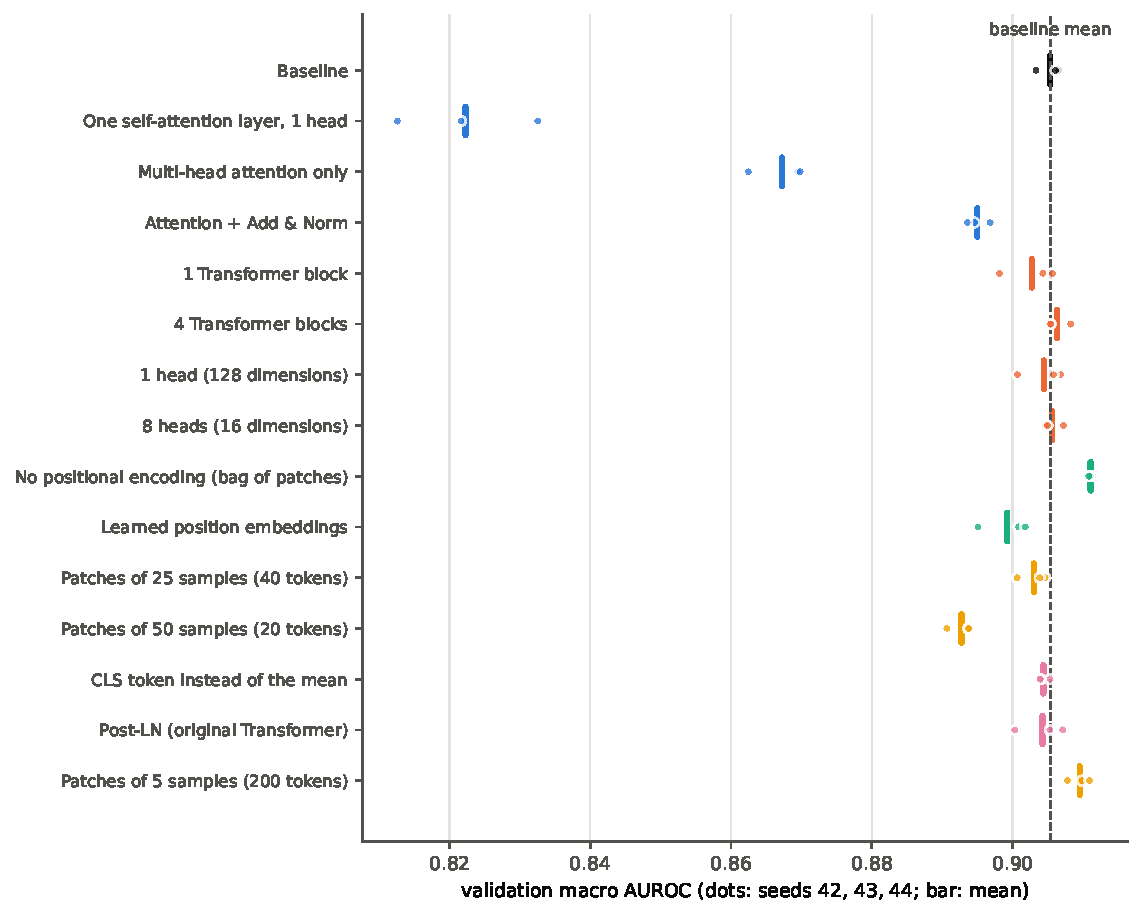
\includegraphics[width=\textwidth,height=0.42\textheight,keepaspectratio]{figures/transformer_ablations.pdf}
\caption[Transformer: ablations]{Transformer ablations: validation macro AUROC (dots: seeds 42, 43, 44; bar: mean; dashed line: baseline mean).}
\label{fig:transformer_ablations}
\end{figure}


\paragraph{Results.}
\begin{enumerate}[leftmargin=1.4em,itemsep=2pt]
  \item \textbf{No model uses the order of the patches.} When the 100 patches of every validation record
        are put in random order, the AUROC changes by at most \transformerOrderDropLayersFour{} in
        absolute value in all fifteen configurations, including those with sinusoidal or learned
        positions (column ``Shuffled''); without positional encoding the change is exactly
        \transformerOrderDropNoPos{}, as it must be. In practice every model here classifies the set of
        100\,ms patches, not their sequence.
  \item \textbf{Hence removing the positional encoding helps} (\transformerDiffMeanNoPos{}, better in
        \transformerNSeedsBetterNoPos{} of \transformerNSeedsComparedNoPos{} seeds) and learned positions
        hurt (\transformerDiffMeanLearnedPos{}, worse in \transformerNSeedsWorseLearnedPos{}). My
        explanation, not tested: if the order is not used, the encoding is only an extra signal added to
        every token that the network must learn to ignore; learned positions add parameters for that
        (\transformerParamsLearnedPos{} against \transformerParamsBase{}) and stop earlier (best epoch
        \onedec{\transformerBestEpochMeanLearnedPos} against \onedec{\transformerBestEpochMeanBase}). Why
        the order does not help is also a hypothesis: the five superclasses may depend mostly on the shape
        of each beat, which a set of patches keeps, while rhythm (RR intervals) would need the order. A
        label set that depends on rhythm would be the test.
  \item \textbf{Heads, depth and readout barely matter beyond one block.} One, four or eight heads differ
        by at most \transformerDiffMeanHeadsOne{} from the baseline; four blocks give
        \transformerDiffMeanLayersFour{} at \onedec{\transformerEpochTimeMeanLayersFour}\,s per epoch
        instead of \onedec{\transformerEpochTimeMeanBase}\,s; a CLS token gives \transformerDiffMeanCls{}.
        None is better or worse in more than one seed.
  \item \textbf{Long patches hurt.} Patches of 50 samples (\transformerTokensPatchFiveZero{} tokens)
        change the AUROC by \transformerDiffMeanPatchFiveZero{} (worse in
        \transformerNSeedsWorsePatchFiveZero{} seeds), patches of 25 by \transformerDiffMeanPatchTwoFive{},
        and patches of 5 (\transformerTokensPatchFive{} tokens) by \transformerDiffMeanPatchFive{}, not
        significant in any seed, at twice the time per epoch. The explanation I propose is the same as for
        the RNN frames, and also a hypothesis: a patch is flattened by one linear layer, so a QRS is seen
        by different weights depending on where it falls inside the patch; shorter patches reduce this.
  \item \textbf{Pre-LN and Post-LN give the same result} (\transformerDiffMeanPostLn{}), but with Post-LN
        the training loss at epoch 5 is higher in \transformerNSeedsTrainLossHigherPostLn{} of
        \transformerNSeedsComparedPostLn{} seeds (\transformerTrainLossEpFiveDiffMeanPostLn{};
        Figure~\ref{fig:transformer_curves}c). This weakly supports the course statement that Pre-LN is
        easier to optimise; with two blocks the effect on the final result is negligible.
  \item \textbf{The baseline overfits early} (Figure~\ref{fig:transformer_curves}a): the validation loss
        reaches its minimum early (best epoch \onedec{\transformerBestEpochMeanBase} on average) and then
        rises while the training loss keeps falling.
\end{enumerate}

% Shared float (common/make_floats.py). Figure: figures/transformer_curves.pdf
\begin{figure}[htbp]
\centering
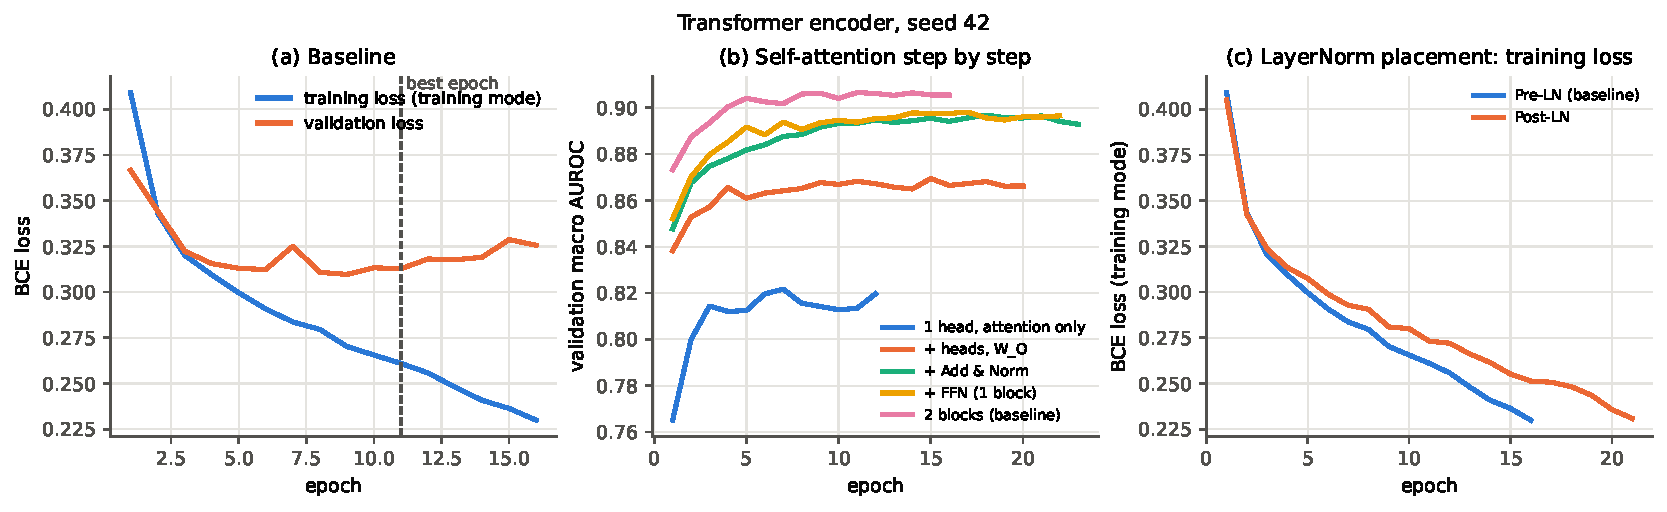
\includegraphics[width=\textwidth,height=0.42\textheight,keepaspectratio]{figures/transformer_curves.pdf}
\caption[Transformer: learning curves and self-attention step by step]{Transformer encoder, seed 42. (a) Baseline losses. (b) Self-attention step by step: validation macro AUROC from one single-head attention layer to two full blocks. (c) Training loss with Pre-LN and Post-LN.}
\label{fig:transformer_curves}
\end{figure}


\paragraph{Where the Transformer looks.} The input sensitivity over the 10\,s is uniform
(Figure~\ref{fig:transformer_time_gradient}): the last 2\,s receive \transformerSensLastNoPos{} of it in
the final model and \transformerSensLastBase{} in the baseline, against \rnnSensLastBase{} for the last
state of the LSTM. This follows from the structure: self-attention and the mean readout treat all
positions alike, with no recurrence that favours recent inputs. The attention statistics
(Table~\ref{tab:transformer_attention}) show how each query spreads its weight. The mean distance between
a query and the patches it attends to is \transformerAttnDistLastNoPos\,s in the last layer of the final
model, the same as with uniform weights (\transformerAttnDistUniformNoPos\,s): attention is not local.
Yet each query concentrates its weight on a few keys: the normalised entropy per query is
\transformerAttnQentropyLastNoPos{} (1 = uniform) and only \transformerAttnQentropyFirstSaSingle{} for the
single head of \texttt{sa\_single}, and the weight on the query's own patch is small
(\transformerAttnDiagLastNoPos{}). Each query looks at a few patches chosen by content, anywhere in the
record, not at its neighbours.

% Shared float (common/make_floats.py). Figure: figures/transformer_time_gradient.pdf
\begin{figure}[htbp]
\centering
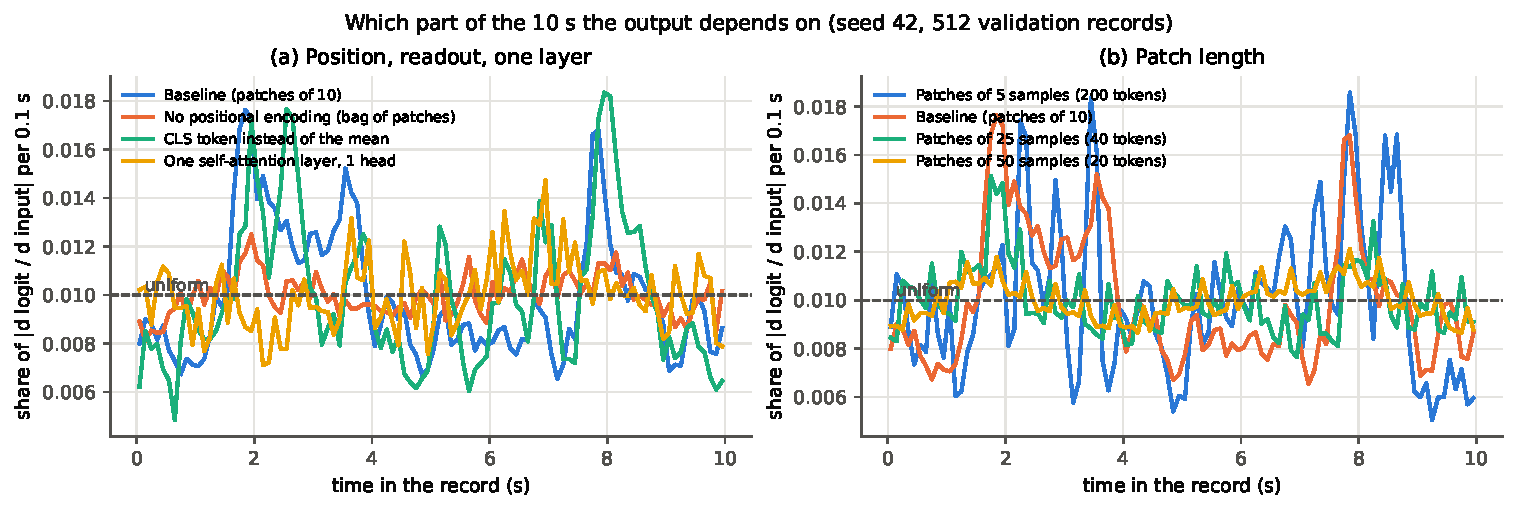
\includegraphics[width=\textwidth,height=0.42\textheight,keepaspectratio]{figures/transformer_time_gradient.pdf}
\caption[Transformer: input sensitivity over time]{Which part of the 10\,s the Transformer output depends on (share of the input gradient per 0.1\,s, seed 42, 512 validation records). (a) Position, readout, one layer. (b) Patch length.}
\label{fig:transformer_time_gradient}
\end{figure}

% Shared float (common/make_floats.py). Table: tables/transformer_attention.tex
\begin{table}[htbp]
\centering
\caption[Transformer: attention statistics]{Attention statistics of the Transformer configurations (seed 42, validation).}
\label{tab:transformer_attention}
\small
\begin{adjustbox}{max width=\textwidth}
% Generated by src/transformer_experiments.py from results/logs/transformer_summary.json.
% Seed-42 model of each configuration, whole validation fold, patch tokens only, heads averaged.
% Distance: mean attention distance in seconds (uniform weights in brackets). Entropy: H / log T (1 = uniform).
% Own patch: weight of each query on its own patch (1/T if uniform). Received: entropy of the attention each patch receives.
\begin{tabular}{lrrcccccc}
\toprule
 & & & \multicolumn{2}{c}{Distance (s)} & \multicolumn{2}{c}{Query entropy} & Own patch & Received \\
\cmidrule(lr){4-5}\cmidrule(lr){6-7}
Configuration & Layers & Tokens & First layer & Last layer (uniform) & First & Last & Last (1/$T$) & Last \\
\midrule
Baseline: Pre-LN, 2 blocks, 4 heads, 100 patches, mean & \transformerAttnLayersBase{} & \transformerAttnTokensBase{} & \transformerAttnDistFirstBase{} & \transformerAttnDistLastBase{} (\transformerAttnDistUniformBase{}) & \transformerAttnQentropyFirstBase{} & \transformerAttnQentropyLastBase{} & \transformerAttnDiagLastBase{} (\transformerAttnUniformBase{}) & \transformerAttnRecvEntropyLastBase{} \\
One self-attention layer, 1 head & \transformerAttnLayersSaSingle{} & \transformerAttnTokensSaSingle{} & \transformerAttnDistFirstSaSingle{} & \transformerAttnDistLastSaSingle{} (\transformerAttnDistUniformSaSingle{}) & \transformerAttnQentropyFirstSaSingle{} & \transformerAttnQentropyLastSaSingle{} & \transformerAttnDiagLastSaSingle{} (\transformerAttnUniformSaSingle{}) & \transformerAttnRecvEntropyLastSaSingle{} \\
Multi-head attention only & \transformerAttnLayersMhsa{} & \transformerAttnTokensMhsa{} & \transformerAttnDistFirstMhsa{} & \transformerAttnDistLastMhsa{} (\transformerAttnDistUniformMhsa{}) & \transformerAttnQentropyFirstMhsa{} & \transformerAttnQentropyLastMhsa{} & \transformerAttnDiagLastMhsa{} (\transformerAttnUniformMhsa{}) & \transformerAttnRecvEntropyLastMhsa{} \\
Attention + Add \& Norm & \transformerAttnLayersNoFfn{} & \transformerAttnTokensNoFfn{} & \transformerAttnDistFirstNoFfn{} & \transformerAttnDistLastNoFfn{} (\transformerAttnDistUniformNoFfn{}) & \transformerAttnQentropyFirstNoFfn{} & \transformerAttnQentropyLastNoFfn{} & \transformerAttnDiagLastNoFfn{} (\transformerAttnUniformNoFfn{}) & \transformerAttnRecvEntropyLastNoFfn{} \\
1 Transformer block & \transformerAttnLayersLayersOne{} & \transformerAttnTokensLayersOne{} & \transformerAttnDistFirstLayersOne{} & \transformerAttnDistLastLayersOne{} (\transformerAttnDistUniformLayersOne{}) & \transformerAttnQentropyFirstLayersOne{} & \transformerAttnQentropyLastLayersOne{} & \transformerAttnDiagLastLayersOne{} (\transformerAttnUniformLayersOne{}) & \transformerAttnRecvEntropyLastLayersOne{} \\
4 Transformer blocks & \transformerAttnLayersLayersFour{} & \transformerAttnTokensLayersFour{} & \transformerAttnDistFirstLayersFour{} & \transformerAttnDistLastLayersFour{} (\transformerAttnDistUniformLayersFour{}) & \transformerAttnQentropyFirstLayersFour{} & \transformerAttnQentropyLastLayersFour{} & \transformerAttnDiagLastLayersFour{} (\transformerAttnUniformLayersFour{}) & \transformerAttnRecvEntropyLastLayersFour{} \\
1 head (128 dimensions) & \transformerAttnLayersHeadsOne{} & \transformerAttnTokensHeadsOne{} & \transformerAttnDistFirstHeadsOne{} & \transformerAttnDistLastHeadsOne{} (\transformerAttnDistUniformHeadsOne{}) & \transformerAttnQentropyFirstHeadsOne{} & \transformerAttnQentropyLastHeadsOne{} & \transformerAttnDiagLastHeadsOne{} (\transformerAttnUniformHeadsOne{}) & \transformerAttnRecvEntropyLastHeadsOne{} \\
8 heads (16 dimensions) & \transformerAttnLayersHeadsEight{} & \transformerAttnTokensHeadsEight{} & \transformerAttnDistFirstHeadsEight{} & \transformerAttnDistLastHeadsEight{} (\transformerAttnDistUniformHeadsEight{}) & \transformerAttnQentropyFirstHeadsEight{} & \transformerAttnQentropyLastHeadsEight{} & \transformerAttnDiagLastHeadsEight{} (\transformerAttnUniformHeadsEight{}) & \transformerAttnRecvEntropyLastHeadsEight{} \\
No positional encoding (bag of patches) & \transformerAttnLayersNoPos{} & \transformerAttnTokensNoPos{} & \transformerAttnDistFirstNoPos{} & \transformerAttnDistLastNoPos{} (\transformerAttnDistUniformNoPos{}) & \transformerAttnQentropyFirstNoPos{} & \transformerAttnQentropyLastNoPos{} & \transformerAttnDiagLastNoPos{} (\transformerAttnUniformNoPos{}) & \transformerAttnRecvEntropyLastNoPos{} \\
Learned position embeddings & \transformerAttnLayersLearnedPos{} & \transformerAttnTokensLearnedPos{} & \transformerAttnDistFirstLearnedPos{} & \transformerAttnDistLastLearnedPos{} (\transformerAttnDistUniformLearnedPos{}) & \transformerAttnQentropyFirstLearnedPos{} & \transformerAttnQentropyLastLearnedPos{} & \transformerAttnDiagLastLearnedPos{} (\transformerAttnUniformLearnedPos{}) & \transformerAttnRecvEntropyLastLearnedPos{} \\
Patches of 25 samples (40 tokens) & \transformerAttnLayersPatchTwoFive{} & \transformerAttnTokensPatchTwoFive{} & \transformerAttnDistFirstPatchTwoFive{} & \transformerAttnDistLastPatchTwoFive{} (\transformerAttnDistUniformPatchTwoFive{}) & \transformerAttnQentropyFirstPatchTwoFive{} & \transformerAttnQentropyLastPatchTwoFive{} & \transformerAttnDiagLastPatchTwoFive{} (\transformerAttnUniformPatchTwoFive{}) & \transformerAttnRecvEntropyLastPatchTwoFive{} \\
Patches of 50 samples (20 tokens) & \transformerAttnLayersPatchFiveZero{} & \transformerAttnTokensPatchFiveZero{} & \transformerAttnDistFirstPatchFiveZero{} & \transformerAttnDistLastPatchFiveZero{} (\transformerAttnDistUniformPatchFiveZero{}) & \transformerAttnQentropyFirstPatchFiveZero{} & \transformerAttnQentropyLastPatchFiveZero{} & \transformerAttnDiagLastPatchFiveZero{} (\transformerAttnUniformPatchFiveZero{}) & \transformerAttnRecvEntropyLastPatchFiveZero{} \\
CLS token instead of the mean & \transformerAttnLayersCls{} & \transformerAttnTokensCls{} & \transformerAttnDistFirstCls{} & \transformerAttnDistLastCls{} (\transformerAttnDistUniformCls{}) & \transformerAttnQentropyFirstCls{} & \transformerAttnQentropyLastCls{} & \transformerAttnDiagLastCls{} (\transformerAttnUniformCls{}) & \transformerAttnRecvEntropyLastCls{} \\
Post-LN (original Transformer) & \transformerAttnLayersPostLn{} & \transformerAttnTokensPostLn{} & \transformerAttnDistFirstPostLn{} & \transformerAttnDistLastPostLn{} (\transformerAttnDistUniformPostLn{}) & \transformerAttnQentropyFirstPostLn{} & \transformerAttnQentropyLastPostLn{} & \transformerAttnDiagLastPostLn{} (\transformerAttnUniformPostLn{}) & \transformerAttnRecvEntropyLastPostLn{} \\
Patches of 5 samples (200 tokens) & \transformerAttnLayersPatchFive{} & \transformerAttnTokensPatchFive{} & \transformerAttnDistFirstPatchFive{} & \transformerAttnDistLastPatchFive{} (\transformerAttnDistUniformPatchFive{}) & \transformerAttnQentropyFirstPatchFive{} & \transformerAttnQentropyLastPatchFive{} & \transformerAttnDiagLastPatchFive{} (\transformerAttnUniformPatchFive{}) & \transformerAttnRecvEntropyLastPatchFive{} \\
\bottomrule
\end{tabular}

\end{adjustbox}
\end{table}


The attention maps (Figures~\ref{fig:transformer_attention} and~\ref{fig:transformer_attention_maps}) are
made of vertical stripes: most queries attend to the same few keys. In the NORM example these keys fall
on the QRS complexes of lead II, one stripe per beat for some heads, and different heads of the last
layer pick different subsets of beats. This alignment is read from the figures only; no number in the
summary measures it, so I state it as an observation, not as a result. Three of the five example records
are missed by the final model, as the probabilities in the column titles show.

% Shared float (common/make_floats.py). Figure: figures/transformer_attention.pdf
\begin{figure}[htbp]
\centering
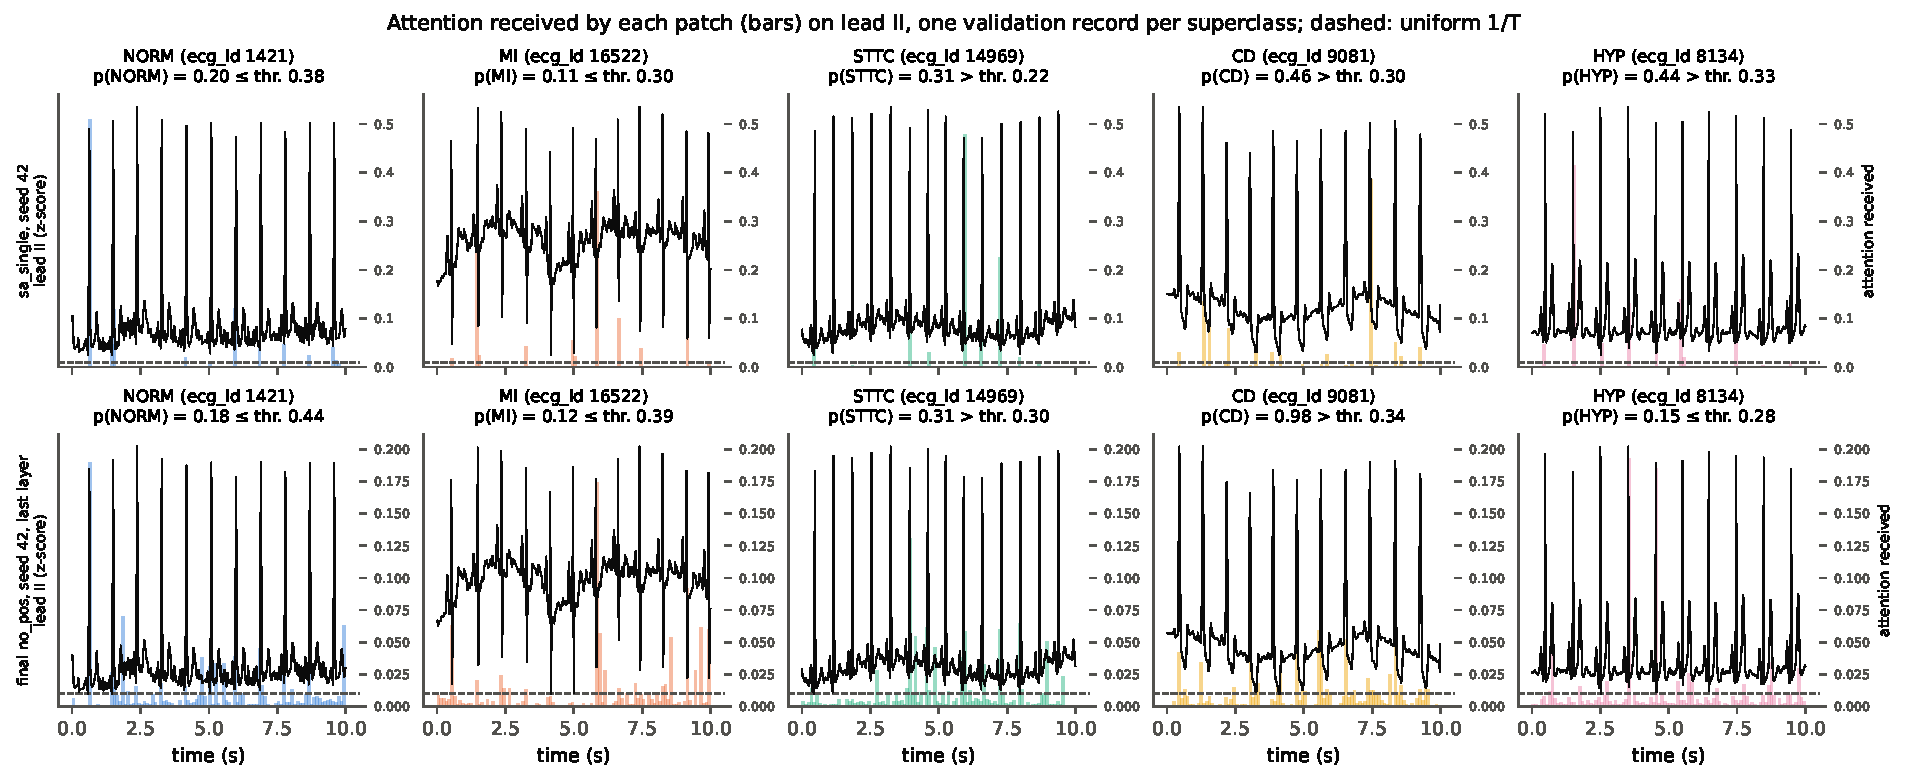
\includegraphics[width=\textwidth,height=0.42\textheight,keepaspectratio]{figures/transformer_attention.pdf}
\caption[Transformer: attention received by each patch]{Attention received by each patch (bars) on lead II, one validation record per superclass: single attention layer (\texttt{sa\_single}, top) and last layer of the final Transformer (\texttt{no\_pos}, bottom). Titles: predicted probability and threshold.}
\label{fig:transformer_attention}
\end{figure}

% Shared float (common/make_floats.py). Figure: figures/transformer_attention_maps.pdf
\begin{figure}[htbp]
\centering
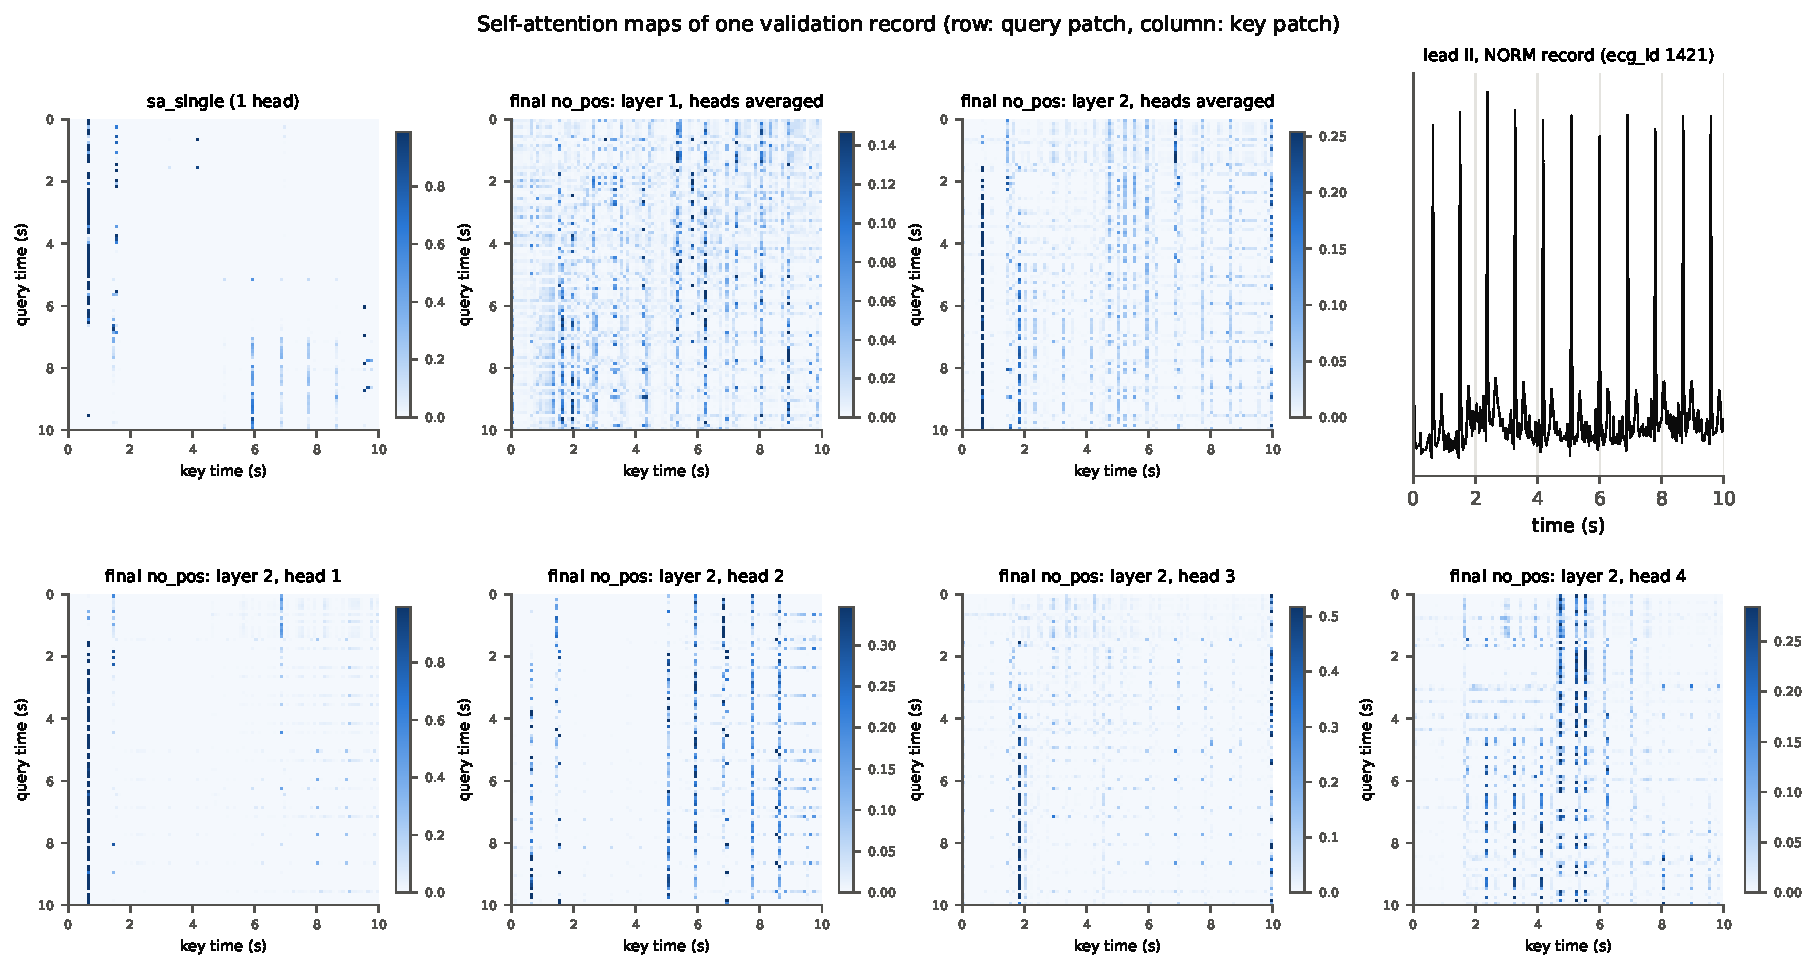
\includegraphics[width=\textwidth,height=0.42\textheight,keepaspectratio]{figures/transformer_attention_maps.pdf}
\caption[Transformer: self-attention maps]{Self-attention maps of one validation NORM record (row: query patch, column: key patch): the single attention layer, both layers of the final Transformer (heads averaged) and the four heads of its last layer.}
\label{fig:transformer_attention_maps}
\end{figure}


\paragraph{Final Transformer.} The rule of D18 selected \texttt{no\_pos}, two Pre-LN blocks without
positional encoding (Table~\ref{tab:transformer_final}). It must be described as what it is: a
permutation-invariant model of the set of 100\,ms patches. On test it reaches
\transformerFinalTestMacroAurocMean{}~$\pm$~\transformerFinalTestMacroAurocSd{}. It is below the CNN
(\transformerDiffCnnMean{}), the final RNN (\transformerDiffRnnMean{}) and the final RNN + attention
(\transformerDiffRnnAttnMean{}), worse in all three seeds against each, and far above the dense network
(\transformerDiffDenseMean{}). On validation it is better than its baseline in all seeds, but only by
\transformerDiffMeanNoPos{}, and it was not compared directly with \texttt{patch5}, whose mean is close
(\transformerValAurocMeanPatchFive{} against \transformerValAurocMeanNoPos{}).

% Shared float (common/make_floats.py). Table: tables/transformer_final.tex
\begin{table}[htbp]
\centering
\caption[Transformer: final model (test)]{Final Transformer (\texttt{no\_pos}) on the test fold, with the final CNN, RNN, RNN + attention, Dense and trivial models.}
\label{tab:transformer_final}
\small
\begin{adjustbox}{max width=\textwidth}
% Generated by src/transformer_experiments.py from results/logs/transformer_summary.json.
% Needs report/numbers.tex (aliases "transformer", "trivial", "cnn", "rnn", "dense").
\begin{tabular}{lccccccc}
\toprule
 & \multicolumn{2}{c}{Transformer (final)} & CNN (final) & RNN (final) & RNN + att.\ (final) & Dense (final) & Trivial \\
\cmidrule(lr){2-3}
Test AUROC & First seed [95\% CI] & Mean $\pm$ SD (seeds) & Mean $\pm$ SD & Mean $\pm$ SD & Mean $\pm$ SD & Mean $\pm$ SD &  \\
\midrule
Macro & \transformerFinalFirstTestMacroAuroc{} [\transformerFinalFirstTestMacroAurocLo{}, \transformerFinalFirstTestMacroAurocHi{}] & \transformerFinalTestMacroAurocMean{} $\pm$ \transformerFinalTestMacroAurocSd{} & \cnnFinalTestMacroAurocMean{} $\pm$ \cnnFinalTestMacroAurocSd{} & \rnnFinalTestMacroAurocMean{} $\pm$ \rnnFinalTestMacroAurocSd{} & \rnnAttnfinalTestMacroAurocMean{} $\pm$ \rnnAttnfinalTestMacroAurocSd{} & \denseFinalTestMacroAurocMean{} $\pm$ \denseFinalTestMacroAurocSd{} & \trivialTestMacroAuroc{} \\
\midrule
NORM & \transformerFinalFirstTestAurocNORM{} [\transformerFinalFirstTestAurocNORMLo{}, \transformerFinalFirstTestAurocNORMHi{}] & \transformerFinalTestAurocNORMMean{} $\pm$ \transformerFinalTestAurocNORMSd{} & \cnnFinalTestAurocNORMMean{} $\pm$ \cnnFinalTestAurocNORMSd{} & \rnnFinalTestAurocNORMMean{} $\pm$ \rnnFinalTestAurocNORMSd{} & \rnnAttnfinalTestAurocNORMMean{} $\pm$ \rnnAttnfinalTestAurocNORMSd{} & \denseFinalTestAurocNORMMean{} $\pm$ \denseFinalTestAurocNORMSd{} & \trivialTestAurocNORM{} \\
MI & \transformerFinalFirstTestAurocMI{} [\transformerFinalFirstTestAurocMILo{}, \transformerFinalFirstTestAurocMIHi{}] & \transformerFinalTestAurocMIMean{} $\pm$ \transformerFinalTestAurocMISd{} & \cnnFinalTestAurocMIMean{} $\pm$ \cnnFinalTestAurocMISd{} & \rnnFinalTestAurocMIMean{} $\pm$ \rnnFinalTestAurocMISd{} & \rnnAttnfinalTestAurocMIMean{} $\pm$ \rnnAttnfinalTestAurocMISd{} & \denseFinalTestAurocMIMean{} $\pm$ \denseFinalTestAurocMISd{} & \trivialTestAurocMI{} \\
STTC & \transformerFinalFirstTestAurocSTTC{} [\transformerFinalFirstTestAurocSTTCLo{}, \transformerFinalFirstTestAurocSTTCHi{}] & \transformerFinalTestAurocSTTCMean{} $\pm$ \transformerFinalTestAurocSTTCSd{} & \cnnFinalTestAurocSTTCMean{} $\pm$ \cnnFinalTestAurocSTTCSd{} & \rnnFinalTestAurocSTTCMean{} $\pm$ \rnnFinalTestAurocSTTCSd{} & \rnnAttnfinalTestAurocSTTCMean{} $\pm$ \rnnAttnfinalTestAurocSTTCSd{} & \denseFinalTestAurocSTTCMean{} $\pm$ \denseFinalTestAurocSTTCSd{} & \trivialTestAurocSTTC{} \\
CD & \transformerFinalFirstTestAurocCD{} [\transformerFinalFirstTestAurocCDLo{}, \transformerFinalFirstTestAurocCDHi{}] & \transformerFinalTestAurocCDMean{} $\pm$ \transformerFinalTestAurocCDSd{} & \cnnFinalTestAurocCDMean{} $\pm$ \cnnFinalTestAurocCDSd{} & \rnnFinalTestAurocCDMean{} $\pm$ \rnnFinalTestAurocCDSd{} & \rnnAttnfinalTestAurocCDMean{} $\pm$ \rnnAttnfinalTestAurocCDSd{} & \denseFinalTestAurocCDMean{} $\pm$ \denseFinalTestAurocCDSd{} & \trivialTestAurocCD{} \\
HYP & \transformerFinalFirstTestAurocHYP{} [\transformerFinalFirstTestAurocHYPLo{}, \transformerFinalFirstTestAurocHYPHi{}] & \transformerFinalTestAurocHYPMean{} $\pm$ \transformerFinalTestAurocHYPSd{} & \cnnFinalTestAurocHYPMean{} $\pm$ \cnnFinalTestAurocHYPSd{} & \rnnFinalTestAurocHYPMean{} $\pm$ \rnnFinalTestAurocHYPSd{} & \rnnAttnfinalTestAurocHYPMean{} $\pm$ \rnnAttnfinalTestAurocHYPSd{} & \denseFinalTestAurocHYPMean{} $\pm$ \denseFinalTestAurocHYPSd{} & \trivialTestAurocHYP{} \\
\midrule
$\Delta$ macro vs.\ CNN, seed 42 & \transformerDiffCnnSFourTwo{} [\transformerDiffCnnLoSFourTwo{}, \transformerDiffCnnHiSFourTwo{}] & & & & & & \\
$\Delta$ macro vs.\ CNN, seed 43 & \transformerDiffCnnSFourThree{} [\transformerDiffCnnLoSFourThree{}, \transformerDiffCnnHiSFourThree{}] & & & & & & \\
$\Delta$ macro vs.\ CNN, seed 44 & \transformerDiffCnnSFourFour{} [\transformerDiffCnnLoSFourFour{}, \transformerDiffCnnHiSFourFour{}] & & & & & & \\
$\Delta$ macro vs.\ RNN, seed 42 & \transformerDiffRnnSFourTwo{} [\transformerDiffRnnLoSFourTwo{}, \transformerDiffRnnHiSFourTwo{}] & & & & & & \\
$\Delta$ macro vs.\ RNN, seed 43 & \transformerDiffRnnSFourThree{} [\transformerDiffRnnLoSFourThree{}, \transformerDiffRnnHiSFourThree{}] & & & & & & \\
$\Delta$ macro vs.\ RNN, seed 44 & \transformerDiffRnnSFourFour{} [\transformerDiffRnnLoSFourFour{}, \transformerDiffRnnHiSFourFour{}] & & & & & & \\
$\Delta$ macro vs.\ RNN + att., seed 42 & \transformerDiffRnnAttnSFourTwo{} [\transformerDiffRnnAttnLoSFourTwo{}, \transformerDiffRnnAttnHiSFourTwo{}] & & & & & & \\
$\Delta$ macro vs.\ RNN + att., seed 43 & \transformerDiffRnnAttnSFourThree{} [\transformerDiffRnnAttnLoSFourThree{}, \transformerDiffRnnAttnHiSFourThree{}] & & & & & & \\
$\Delta$ macro vs.\ RNN + att., seed 44 & \transformerDiffRnnAttnSFourFour{} [\transformerDiffRnnAttnLoSFourFour{}, \transformerDiffRnnAttnHiSFourFour{}] & & & & & & \\
$\Delta$ macro vs.\ Dense, seed 42 & \transformerDiffDenseSFourTwo{} [\transformerDiffDenseLoSFourTwo{}, \transformerDiffDenseHiSFourTwo{}] & & & & & & \\
$\Delta$ macro vs.\ Dense, seed 43 & \transformerDiffDenseSFourThree{} [\transformerDiffDenseLoSFourThree{}, \transformerDiffDenseHiSFourThree{}] & & & & & & \\
$\Delta$ macro vs.\ Dense, seed 44 & \transformerDiffDenseSFourFour{} [\transformerDiffDenseLoSFourFour{}, \transformerDiffDenseHiSFourFour{}] & & & & & & \\
$\Delta$ macro vs.\ trivial, seed 42 & \transformerDiffTrivialSFourTwo{} [\transformerDiffTrivialLoSFourTwo{}, \transformerDiffTrivialHiSFourTwo{}] & & & & & & \\
$\Delta$ macro vs.\ trivial, seed 43 & \transformerDiffTrivialSFourThree{} [\transformerDiffTrivialLoSFourThree{}, \transformerDiffTrivialHiSFourThree{}] & & & & & & \\
$\Delta$ macro vs.\ trivial, seed 44 & \transformerDiffTrivialSFourFour{} [\transformerDiffTrivialLoSFourFour{}, \transformerDiffTrivialHiSFourFour{}] & & & & & & \\
\bottomrule
\end{tabular}

\end{adjustbox}
\end{table}


% ---------------------------------------------------------------------
\subsection{What the architectures show together}\label{sec:arch-summary}

On the same task, data and protocol, the four families with shared weights rank CNN
(\cnnFinalTestMacroAurocMean{}), RNN (\rnnFinalTestMacroAurocMean{}), RNN + attention
(\rnnAttnfinalTestMacroAurocMean{}) and Transformer (\transformerFinalTestMacroAurocMean{}), all far
above the dense network (\denseFinalTestMacroAurocMean{}); per class, the Transformer's largest gaps to
the CNN are in CD and MI (Table~\ref{tab:transformer_final}). Three conclusions come out of my blocks.
First, the large step is from no weight sharing to any weight sharing over time; the differences among
the families that share weights are much smaller than their common gap to the dense network
(Table~\ref{tab:comparison_final}). Second, local feature extraction is
what the ECG rewards most here: the best recurrent model has a convolutional front end, raw samples beat
flattened frames, and short patches beat long ones. Third, the mechanisms that make recurrence and
attention powerful on language, long memory and order, were not used by this task: attention pooling
behaved like a mean, and no Transformer used the order of the patches. This is a statement about this
dataset and these five labels, not about the architectures in general.
